\subsubsection{Dataset Curation Details}
\label{app:dataset_curation_details}

\subsubsection{Training data curation.}
\label{app:training_curation}
Training problems were sourced from two advanced textbooks featuring graduate-level and Olympiad-style inequality proof problems. We parsed these textbooks to extract proof problems, their step-wise solutions, and relevant theorems.
We developed two LLM-based rephrasers to transform each source problem into two sub-tasks defined in  \S\ref{sec:task_formalization}: bound estimation and relation prediction. For instance, a source problem like ``Prove $a + b \geq 2\sqrt{ab}$ for $\forall a, b \in \mathbb{R}^{+}$'' would be rephrased into a bound estimation task (e.g., ``Determine the maximal constant $C$ such that $a + b \geq C\sqrt{ab}$ holds for $\forall a, b \in \mathbb{R}^{+}$'') and a relation prediction task (e.g., ``Determine the inequality relation in the expression $a + b ~ (~) ~ 2\sqrt{ab}$ that holds for $\forall a, b \in \mathbb{R}^{+}$'').

Crucially, while rephrased problems are altered from the source proof problem in the format, they preserve the core mathematical reasoning and solution steps—such as applying relevant theorems, determining boundary conditions, and verifying inequalities. An annotation tool (see \S\ref{app:data_annotation_tool}) was developed to facilitate human expert review and correction of the LLM-rephrased problems.
Extracted theorems were curated, each including its name, a natural language definition, and a list of training problems where it is applicable.


% \clearpage
\subsubsection{Data Annotation Tool}
\label{app:data_annotation_tool}

\begin{figure}[ht]
    \centering
    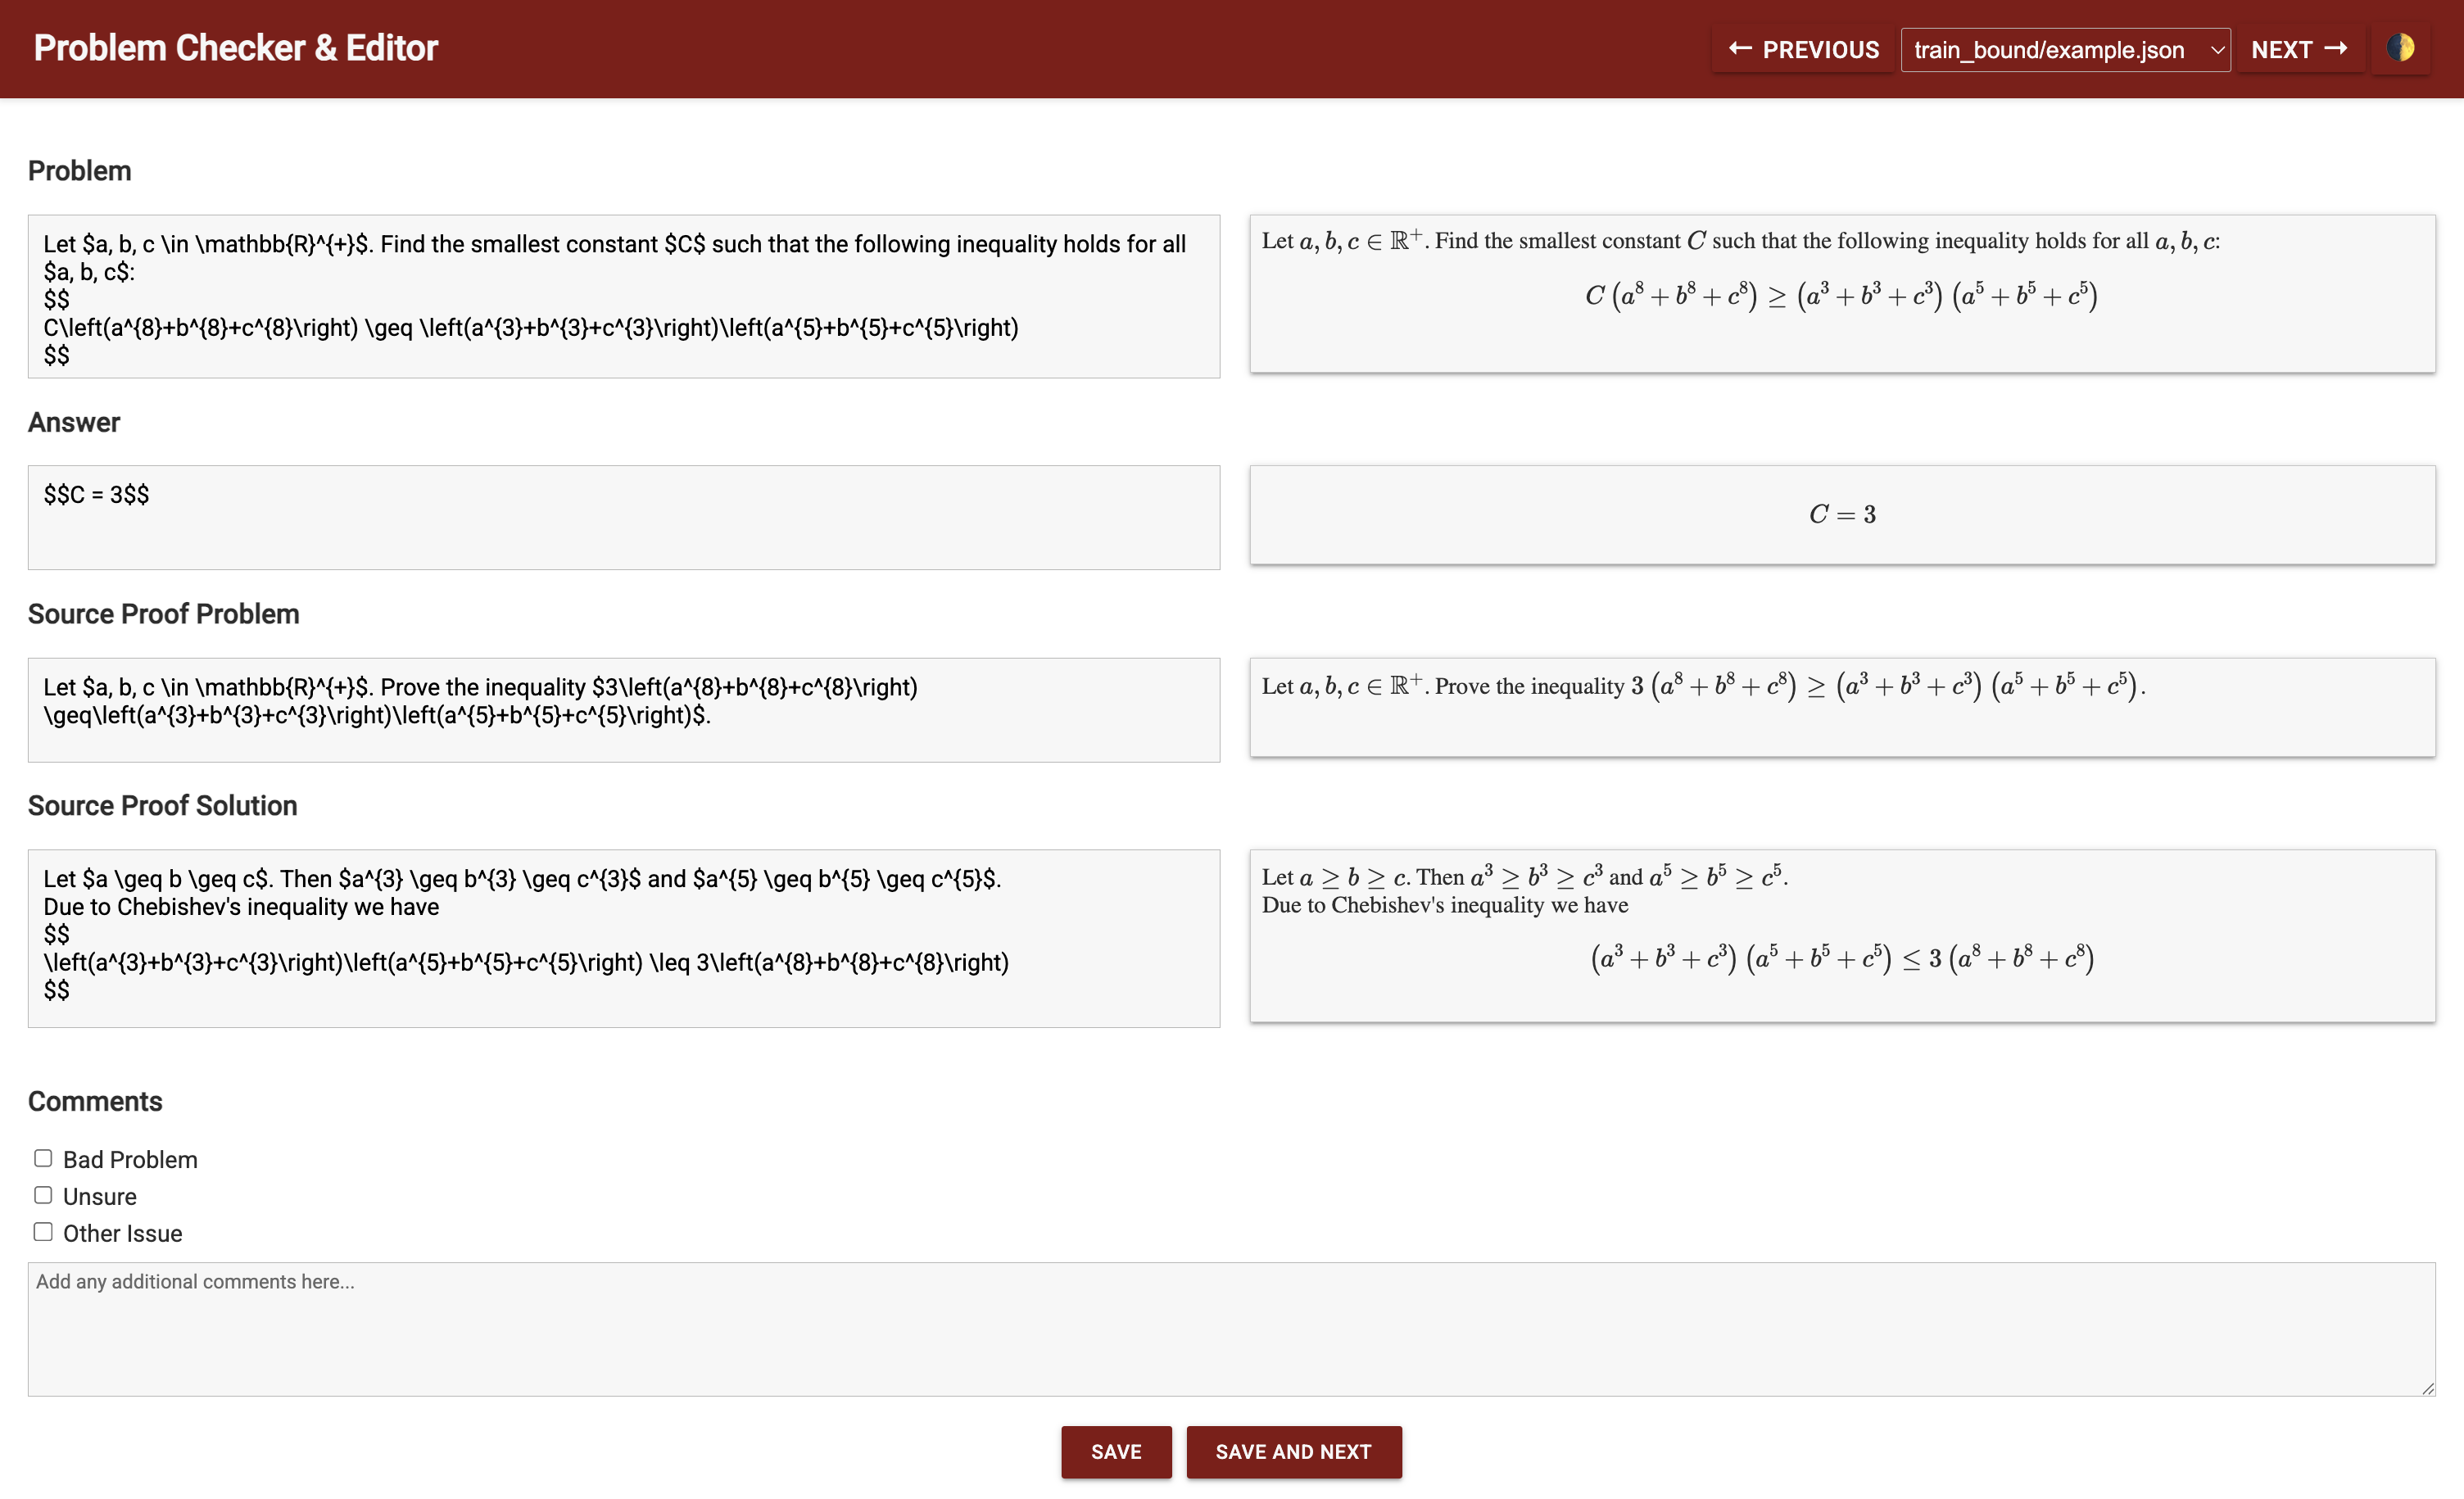
\includegraphics[width=1\linewidth]{figs/data_annot_tool_bound.png}
    \caption{The interface of our developed tool for checking and editing the bound problems.}
    \label{fig:data_annot_tool_bound}
\end{figure}

\begin{figure}[ht]
    \centering
    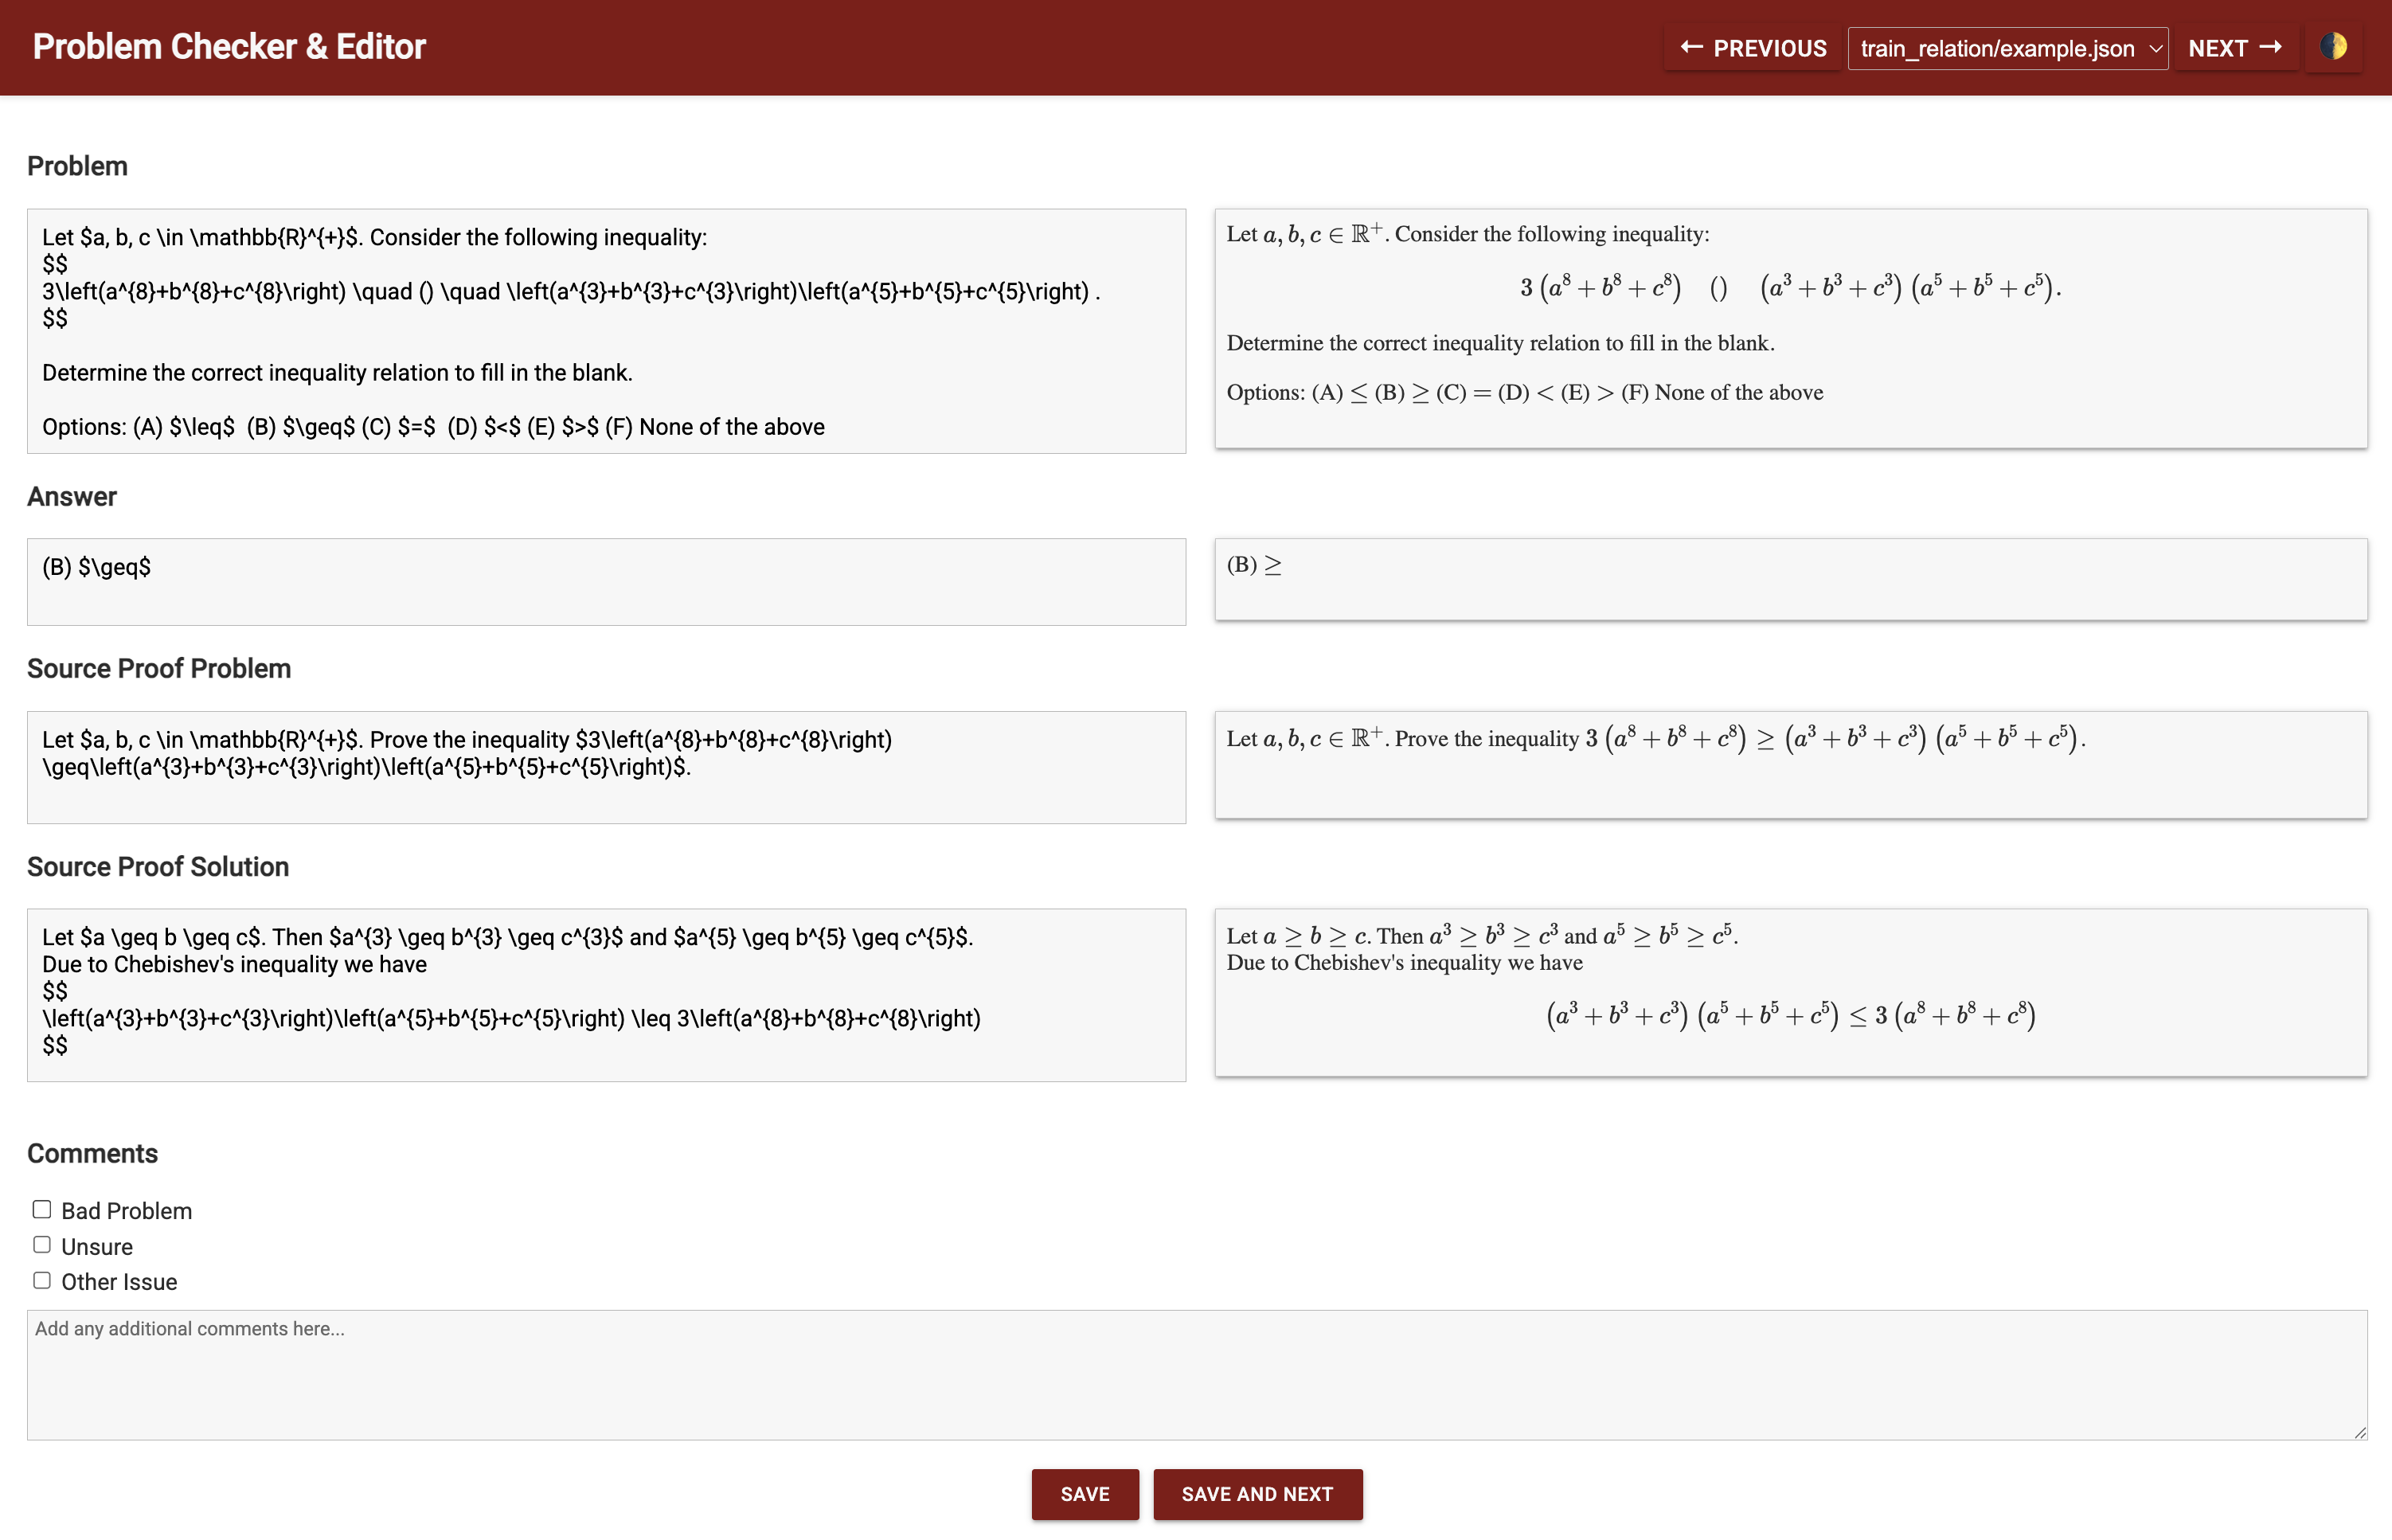
\includegraphics[width=1\linewidth]{figs/data_annot_tool_relation.png}
    \caption{The interface of our developed tool for checking and editing the relation problems.}
    \label{fig:data_annot_tool_relation}
\end{figure}


\newpage
\subsubsection{Prompts for Rephrasing Problems}
\label{app:prompt_rephrasing_problem}

% Prompt for Rephrasing Problems
\begin{textcolorbox}[Prompt for Rephrasing Proofs to Bound Problems]
\textbf{Task:} Transform the given inequality problem into a bound prediction problem by introducing a constant C and determining its optimal value.
\\\\
\textbf{Instructions:}

1. Analyze the original problem, focusing on its structure and potential for transformation. \\
2. Introduce a constant $C$ by either replacing an existing constant or creating a new relationship between expressions. \\
3. Determine whether to find the minimal or maximal value of $C$ that satisfies the inequality for all relevant variables. \\
4. Consider factors such as homogeneity, existing constraints, and the domain of variables (e.g., positive reals, all reals). \\
5. Ensure the rephrased problem maintains the mathematical essence and constraints of the original. \\

\textbf{Output Format:}

Provide your response in the following structure:

\texttt{<Analysis>}: Concise explanation of key features and transformation approach. \\
\texttt{<Conclusion>}: YES or NO, followed by a brief summary of the transformation. \\
\texttt{<Rephrased Problem>}: Transformed problem statement, focusing on finding the optimal $C$. \\
\texttt{<Answer>}: $C = <value>$.
\\\\
\textbf{Key Considerations:} \\
1. For double inequalities, attempt to rephrase as a single bound prediction problem when possible. \\
2. In homogeneous inequalities, focus on the ratios between variables rather than their absolute values. \\
3. Incorporate any existing constraints into the rephrased version of the problem. \\
4. Clearly specify the domain of the variables in the rephrased problem statement. \\
5. Ensure that the rephrased problem is logically equivalent to the original.
\\\\
\textbf{Example:} \\
% \texttt{\{examples\}}
Original problem:
Let $a, b, c \in \mathbb{R}^{+}$. Prove the inequality
$$
\frac{a b c}{(1+a)(a+b)(b+c)(c+16)} \leq \frac{1}{81}
$$

\vspace{2mm}
\texttt{<Analysis>}: To turn this into a bound prediction problem, we can focus on the following steps: \\
1. The left side is a rational expression that is always positive for $a, b, c \in \mathbb{R}^{+}$. \\
2. The right side is a fixed constant $\frac{1}{81}$.\\
3. We replace the constant $\frac{1}{81}$ with a variable $C$ and ask: What is the smallest $C$ such that the inequality holds for all positive $a, b, c$?\\
4. This approach allows us to determine the tightest possible upper bound for the left-hand expression.\\
5. If we find the smallest $C$ that works, we prove the original inequality and show it's the best possible.

\vspace{2mm}
\texttt{<Conclusion>}: YES, the inequality can be rephrased as a bound prediction problem. By replacing the constant $\frac{1}{81}$ with a variable $C$, we can determine the tightest upper bound for the given rational expression, effectively proving the original inequality and demonstrating its optimality.

\vspace{2mm}
\texttt{<Rephrased problem>}: \\
Coll  Determine the minimal constant $C$ such that the following inequality holds for all $a, b, c$:
$$
\frac{abc}{(1+a)(a+b)(b+c)(c+16)} \leq C.
$$
\texttt{<Answer>:} $C = \frac{1}{81}$.
\\\\
\textbf{Now, please rewrite the following problem:}

Original problem: \texttt{\{problem\}}
\end{textcolorbox}
\begin{textcolorbox}[Prompt for Rephrasing Proofs to Relation Problems]
\textbf{Task:} Transform the given inequality proof problem into a relation prediction problem.
\\\\
\textbf{Instructions:}

1. Analyze the original problem, identifying key components such as variables, domains, conditions, and the main inequality. \\
2. Rephrase the problem by maintaining the original expressions and replacing the relation symbol with a blank to be filled. \\
3. Preserve any additional conditions or constraints from the original problem in your rephrased version. \\
4. Change the task from ``Prove'' to ``Determine the correct inequality relation to fill in the blank.'' \\
5. Provide a set of options for the relation, always including $\leq$, $\geq$, $=$, $<$, $>$, and ``None of the above''. \\
6. Determine the correct answer based on your modification and analysis. \\

\textbf{Output Format:}

Provide your response in the following structure:

\vspace{2mm}
\texttt{<Analysis>}: Detailed step-by-step analysis of the original problem and your approach to rephrasing it.

\vspace{2mm}
\texttt{<Conclusion>}: YES or NO, followed by a brief explanation of whether and how the problem can be effectively rephrased.

\vspace{2mm}
\texttt{<Rephrased Problem>}: 

\quad Transformed problem statement.

\quad Options:
(A) $\leq$ \quad
(B) $\geq$\quad
(C) $=$ \quad
(D) $<$ \quad
(E) $>$ \quad
(F) None of the above

\vspace{2mm}
\texttt{<Answer>}: Option letter.
\\\\
\textbf{Key Considerations:} \\
1. Maintain the original mathematical expressions and any given conditions as much as possible.\\
2. Ensure the rephrased problem captures the essence and complexity of the original problem.\\
3. For problems with multiple inequalities, focus on one main inequality for the relation prediction task.\\
4. When dealing with complex fractions or expressions, keep them intact to maintain the problem's difficulty level.\\
5. If the relation depends on specific values of the variables or cannot be definitively determined, consider using ``None of the above'' as the correct answer.
% 6. Use LaTeX format ($$) for all variables and formulas, not \\( and \\).
% ations, use double dollar signs ($$) on separate lines.
\\\\
\textbf{Example:} \\
% \texttt{\{examples\}}
Original problem:
Let $a, b, c \in \mathbb{R}^{+}$. Prove the inequality
$$
\frac{a b c}{(1+a)(a+b)(b+c)(c+16)} \leq \frac{1}{81}
$$
\vspace{2mm}
\texttt{<Analysis>}: To rephrase it to a relation prediction problem, we can focus on the following steps: \\
1. The original problem is a proof task for an inequality involving positive real numbers $a$, $b$, and $c$. \\
2. The left side of the inequality is a complex fraction $\frac{a b c}{(1+a)(a+b)(b+c)(c+16)}$. \\
 % with a product in the numerator and a product of sums in the denominator
3. The right side is a constant fraction $\frac{1}{81}$. \\
4. The original inequality uses the ``less than or equal to'' ($\leq$) relation, which needs to hold for all positive real values of $a$, $b$, and $c$. \\
5. We can transform the proof task into determining the correct relation between the left and right sides of the inequality.

\vspace{2mm}
\texttt{<Conclusion>}: YES, the inequality can be effectively rephrased as a relation prediction problem.

\vspace{2mm}
\texttt{<Rephrased problem>}: \\
Let $a, b, c \in \mathbb{R}^{+}$. Consider the following inequality:
$$
\frac{a b c}{(1+a)(a+b)(b+c)(c+16)} \quad (\quad) \quad \frac{1}{81} .
$$
Determine the correct inequality relation to fill in the blank. 
\\
Options:
(A) $\leq$ \quad
(B) $\geq$\quad
(C) $=$ \quad
(D) $<$ \quad
(E) $>$ \quad
(F) None of the above

\vspace{2mm}
\texttt{<Answer>:} A
\\\\
\textbf{Now, please rewrite the following problem:}

Original problem: \texttt{\{problem\}}
\end{textcolorbox}


% \clearpage
\subsubsection{Benchmark Examples}
\label{app:dataset_examples}

\begin{examplebox}[\dataset Testing Example 1: Bound Problem]
\textbf{Question:} Let $x, y, z > 0$ such that $x+y+z=1$. Determine the minimal constant $C$ such that the following inequality holds for all $x, y, z$:
$$x y(y+4 z)+y z(z+4 x)+z x(x+4 y) \leq C.$$
\end{examplebox}

\begin{examplebox}[\dataset Testing Example 2: Bound Problem]
\textbf{Question:} Let $a_1, a_2, \ldots, a_n$ be real numbers and $S$ be a non-empty subset of $\{1,2, \ldots, n\}$. Find the largest constant $C$ such that the following inequality holds for all $a_1, a_2, \ldots, a_n$ and $S$:
$$
2C \left(\sum_{i \in S} a_i\right)^2 \leq \sum_{1 \leq i \leq j \leq n}\left(a_i+\cdots+a_j\right)^2.
$$
\end{examplebox}

\begin{examplebox}[\dataset Testing Example 3: Bound Problem]
\textbf{Question:} Let $a_1, a_2, \ldots, a_n > 0$ such that $a_1 + a_2 + \ldots + a_n < 1$. Determine the minimal constant $C$ such that the following inequality holds for all $a_1, a_2, \ldots, a_n$:
$$
\frac{a_1 \cdot a_2 \ldots a_n \left(1 - a_1 - a_2 - \ldots - a_n\right)}{\left(a_1 + a_2 + \ldots + a_n\right)\left(1-a_1\right)\left(1-a_2\right) \ldots \left(1-a_n\right)} \leq C\frac{3}{n^{n-1}}.
$$
\end{examplebox}

\clearpage
\begin{examplebox}[\dataset Testing Example 4: Relation Problem]
\textbf{Question:} Let $a, b, c, x, y, z \in \mathbb{R}$ be real numbers such that $a + b + c = 1$ and $x^2 + y^2 + z^2 = 1$. Consider the following expression:
$$
a(x+b) + b(y+c) + c(z+a)  \quad (\quad) \quad 1.
$$
Determine the correct inequality relation to fill in the blank.\\

\textbf{Options:} (A) $\leq$ \quad(B) $\geq$ \quad (C) $=$  \quad (D) $<$ \quad  (E) $>$  \quad (F) None of the above

\end{examplebox}

\begin{examplebox}[\dataset Testing Example 5: Relation Problem]
\textbf{Question:} In the plane of the acute-angled triangle $\triangle ABC$, let $L$ be a line such that $u, v, w$ are the lengths of the perpendiculars from $A, B, C$ respectively to $L$. Consider the following inequality:
$$
u^2 \tan A + v^2 \tan B + w^2 \tan C \quad (\quad) \quad \Delta.
$$
where $\Delta$ is the area of the triangle. Determine the correct inequality relation to fill in the blank.\\

\textbf{Options:} (A) $\leq$ \quad(B) $\geq$ \quad (C) $=$  \quad (D) $<$ \quad  (E) $>$  \quad (F) None of the above

\end{examplebox}

\begin{examplebox}[\dataset Testing Example 6: Relation Problem]
\textbf{Question:} Let $a, b, c$ be the sides of any triangle. Consider the following inequality:
$$
3\left(\sum_{cyc} a b\left(1+2 \cos (c)\right)\right) \quad (\quad) \quad   2\left(\sum_{cyc} \sqrt{\left(c^2+a b(1+2 \cos (c))\right)\left(b^2+a c(1+\cos (b))\right)}\right).
$$
Determine the correct inequality relation to fill in the blank.\\

\textbf{Options:} (A) $\leq$ \quad(B) $\geq$ \quad (C) $=$  \quad (D) $<$ \quad  (E) $>$  \quad (F) None of the above

\end{examplebox}


\clearpage
\subsection{Fine-grained Informal Judge Details}
\label{app:evaluation_details}

\subsubsection{Final Answer Judge}
\label{app:answer_judge_appendix}

\begin{textcolorbox}[Prompt for Final Answer Judge: Answer Extraction for Bound problems]

You are an expert in extracting numbers from answer sentences. 
Below are examples of sentences and the corresponding numbers:\\

Example 1: answer is $C=2$. \\
Answer: $C=2$ \\

Example 2: answer is $C = \frac{1}{\sqrt{2}}$. \\
Answer: $C = \frac{1}{\sqrt{2}}$ \\

Example 3: answer is $\boxed{C=2}$.\\
Answer: $C=2$ \\

Now, extract the number from the following sentence:
\texttt{\{answer\_sentence}\}. \\

Make sure to return the answer in the format as ``\texttt{C=<extracted\_answer>}'', where \texttt{<extracted\_answer>} is the extracted number or expression.
\end{textcolorbox}


\begin{textcolorbox}[Prompt for Final Answer Judge: Answer Extraction for Relation Problems]
You are an expert in extracting option letters (A, B, C, D, E, F) from answer sentences. \\

The options are given below:\\
A: (A) $\leq$ \\
B: (B) $\geq$ \\
C: (C) $=$ \\
D: (D) $<$\\
E: (E) $>$\\
F: (F) None of the above\\

Below are examples of sentences and the corresponding option letters:\\

Example 1: answer is (B) $\geq$. \\
Answer: B\\

Example 2: answer is (E) >. \\
Answer: E\\

Example 3: answer is: $\boxed{\leq}$. \\
Answer: A\\

Now, extract the option letter from the following sentence: \texttt{\{answer\_sentence\}}. \\

Make sure to return the option letter only, without any other characters.
\end{textcolorbox}


\begin{textcolorbox}[Prompt for Final Answer Judge: Answer Equivalence Verification]
You are an expert in verifying mathematical expression equivalence. Analyze if two expressions are exactly equivalent by following these strict rules:\\

\textbf{Required Analysis Steps:}\\
1. Check if both expressions are valid mathematical forms.\\
2. If either expression is not mathematical (e.g., text or undefined), return \texttt{False}.\\
3. For numerical expressions:

\quad - Direct equality (e.g., 2 = 2) → \texttt{True}.

\quad - Different representations of same value (e.g., $1/2$ = $0.5$, $\sqrt{4}$ = $2$) → \texttt{True}.

\quad - Decimal approximations vs exact values (e.g., $2\pi \neq 6.28318$) → \texttt{False}.

4. For algebraic expressions:

\quad - Must have clear, valid transformation path between forms.

\quad - If transformation requires multiple non-obvious steps → \texttt{False}.

\quad - Verify equivalence through algebraic proof when possible.

\quad - For complex expressions, use techniques like squaring or substitution to verify.
\\\\
\textbf{Equivalence Criteria:}

\quad - Must have exactly same deterministic value.

\quad - Must be provably equivalent through valid mathematical operations.

\quad - Different notations of same exact value are equivalent.

\quad - Decimal approximations are NOT equivalent to exact expressions.

\quad - No rounding or approximations allowed.

\quad - If equivalence cannot be conclusively proven → \texttt{False}.
\\\\
\textbf{Example Pairs and their Analysis:}

Ground truth: $C=2$\\
Prediction: $C=2$\\
Analysis: The expressions are identical in both form and value, representing the same integer 2.\\
Equivalent: \texttt{True}\\

Ground truth: $C=1.5$\\
Prediction: $C=\frac{3}{2}$\\
Analysis: The decimal $1.5$ and fraction $\frac{3}{2}$ are different representations of the same number ($1.5 = \frac{3}{2}$).\\
Equivalent: \texttt{True}\\

Ground truth: $C=2\pi$\\
Prediction: $C=6.28318530718$\\
Analysis: While $6.28318530718$ is a decimal approximation of $2\pi$, they are not symbolically equivalent expressions.\\
Equivalent: \texttt{False}\\

Ground truth: $C=\sqrt{\frac{1}{6}}$\\
Prediction: $C=\frac{1}{\sqrt{6}}$\\
Analysis: These are equivalent through the property $\sqrt{\frac{a}{b}} = \frac{\sqrt{a}}{\sqrt{b}}$ when $a,b > 0$.\\
Equivalent: \texttt{True}\\

Ground truth: $C=\sqrt{\frac{3}{2}}$\\
Prediction: $C=\frac{3}{2\sqrt{2}}$\\
Analysis: The expressions differ as proven when squared: $(\sqrt{\frac{3}{2}})^2 = \frac{3}{2} \neq \frac{9}{8} = (\frac{3}{2\sqrt{2}})^2$.\\
Equivalent: \texttt{False}\\

\textbf{Now analyze these expressions:}\\
Ground truth: \texttt{{\{ground\_truth\}}} \\
Prediction: \texttt{{\{prediction\}}}
\end{textcolorbox}

% \clearpage
\subsubsection{Toy Case Judge}
\label{app:toy_case_appendix}

\begin{textcolorbox}[Prompt for Toy Case Judge]
\textbf{Task:} Evaluate the logical rigor of a solution to an inequality problem, focusing specifically on whether the direction of the inequality was justified using toy cases or special value substitution.\\

\textbf{Instructions:}

1. Carefully read the reasoning process used to solve the inequality.

2. Identify whether the direction of the inequality was determined by testing special values, trying toy cases, or relying on extreme-case analysis, rather than providing a general proof valid over the entire domain.

3. If the model uses a toy case (e.g., setting a variable to 0, 1, or choosing symmetric/equal values) or considers a variable tending to 0 or $\infty$ (extreme-case reasoning) to conclude the inequality direction, this should be flagged as logically unsound unless it is later supported by a rigorous or general argument.

4. Substituting special values for the purpose of verifying equality or testing sharpness is acceptable and should not be flagged.

5. If a toy case is used to show that the inequality does not hold (i.e., the two sides are incomparable), this is acceptable and should not be flagged.

6. Trying toy cases or substituting special values for the purpose of exploring or analyzing the problem—without using them to directly conclude the inequality direction—is acceptable and should not be flagged.

7. The goal is to confirm whether the final conclusion is justified for \textit{all variables in the given domain} by using sound and formal reasoning.\\

\textbf{Output Format:}

\texttt{<Analysis>:} Brief explanation of whether toy cases, special values, or extreme-case reasoning were used to justify inequality direction, and whether this undermines the rigor of the proof.\\
\texttt{<Flagged Reasoning Step (if applicable)>:} Quote or summarize the step(s) where toy cases or extreme cases were used to justify the inequality.\\
\texttt{<Answer>:} \texttt{True} or \texttt{False}. It indicates whether the solution's reasoning is logically valid (\texttt{True}) or contains flaws due to unjustified use of toy cases, special value substitution, or extreme-case reasoning (\texttt{False}).\\

\textbf{Key Considerations:}

1. Check which steps are used to justify the final general conclusion.

2. Toy case examples should not be used to conclude general inequality directions.

3. These techniques are allowed for illustration or equality testing, but not as a replacement for a full justification.

4. Extreme-case analysis used as a substitute for proof to justify the final general conclusion should be flagged.

5. Do not provide improvement suggestions---simply judge whether the logic used is valid or flawed.

6. Only reasoning steps that fail to generalize and are used to justify the final general conclusion should be flagged.\\

\textbf{Examples of Inputs and Outputs:}

\texttt{\{examples\}}\\

\textbf{Now analyze the following problem and solution:}

Original Problem:
\texttt{\{query\}}

Solution:
\texttt{\{response\}}

\end{textcolorbox}




\begin{examplebox}[Judge Example 1: Toy Case]
\textbf{Response:}

Let's test the specific values.

\texttt{Case 1:} If \( a = b = c \), then:
\[
\left(\frac{a}{b+c}\right)^2 + \frac{b}{c+a} + \left(\frac{c}{a+b}\right)^2 = \frac{1}{4} + \frac{1}{2} + \frac{1}{4} = 1.
\]

\texttt{Case 2:} If \( a = 0 \) and \( b = c = 1 \), then:

\[
\left(\frac{a}{b+c}\right)^2 + \frac{b}{c+a} + \left(\frac{c}{a+b}\right)^2 = 0 + 1 + 1 = 2.
\]

\wrong{From the test cases, we can conclude that the minimum value of the expression was 1. Therefore, the expression is always at least 1.} The answer is \( \boxed{C = 1 }\).\\

\textbf{Judge Output:}

\texttt{<Analysis>:} The minimum of the expression is derived from two special cases(i.e. $a=b=c$ and $a=0,\,b=c=1$). This is incorrect as it substitutes generality with selected toy cases.   \\

\texttt{<Flagged Reasoning Step (if applicable)>}: \flagged{From the test cases, we can conclude that the minimum value of the expression is 1. Therefore, the expression is always at least 1.} \\

\texttt{<Answer>:} \textbf{\boxed{False}}

\end{examplebox}


% \newpage
\subsubsection{Logical Gap Judge}
\label{app:logical_gap_appendix}

\begin{textcolorbox}[Prompt for Logical Gap Judge]
\textbf{Task:} Evaluate the logical rigor of a proposed solution to a mathematical inequality problem. Focus on whether the reasoning includes non-trivial claims made without justification, logical leaps, or unsupported assertions, while allowing for valid optimization-based, algebraic, or analytic analysis when properly demonstrated.
This prompt does not evaluate whether the direction of an inequality was justified using toy cases, special values, or asymptotic behavior; that aspect is handled separately. \\

\textbf{Instructions:}

1. Carefully read the entire reasoning process used to solve the inequality.

2. Identify whether the solution includes:

\quad - Any non-obvious (non-trivial) claims or transformations without justification or explanation.

\quad - Any logical gaps or skipped steps that lead to intermediate or final conclusions.\\
3. All significant transformations—especially involving inequalities, bounds, or extremal behavior—must be supported by: algebraic manipulation, well-known identities or theorems, valid analytical tools (e.g., convexity, derivatives, limits) or step-by-step numeric or symbolic reasoning.

4. Optimization methods (e.g., Lagrange multipliers, derivative-based analysis) are valid only if the analysis is explicitly shown:

\quad - If a solution invokes optimization or analytical techniques, it must demonstrate key steps, derivative conditions, or critical point verification.

\quad - Statements such as ``solving the constrained optimization problem confirms...'' without any derivation or argument are considered unjustified.

\quad - You do not need to assess whether toy cases, special values, or extreme behavior were used to infer the inequality direction. That responsibility lies outside the scope of this Judge.\\
5. Simple algebra or widely known transformations (e.g., AM-GM, factoring identities) may be used without full derivation.\\
6. The goal is to assess whether each important conclusion within the reasoning—not just the final answer—is logically supported and rigorously justified.\\

\textbf{Output Format:}

\texttt{<Analysis>:} Step-by-step explanation of whether the reasoning is logically sound. Highlight any unjustified claims or skipped steps, unless they are supported by valid asymptotic, numeric, or analytic reasoning. \\
\texttt{<Flagged Reasoning Step (if applicable)>:} Quote or summarize the specific step(s) where an unjustified claim or logical leap occurred. \\
\texttt{<Answer>:} \texttt{True} or \texttt{False}. \texttt{True} if the reasoning is valid; \texttt{False} if it contains unjustified steps or unsupported claims. \\

\textbf{Key Considerations:}

1. Focus on whether each major step (not just the final answer) is logically justified.\\
2. Non-trivial algebraic identities or inequality steps must be explained unless they are well-known.\\
3. Minor simplifications and standard techniques are acceptable without proof.\\
4. Do not flag steps involving toy cases, extreme values, or special substitutions used to infer inequality direction—those are out of scope here.\\
5. Claims like ``a numerical check shows'' must include specific values, results, or graphs to be valid.\\
6. Optimization-based arguments (e.g., Lagrange multipliers, critical point methods) must include demonstrated steps or analytic structure. If only the method is named but not applied, the reasoning should be flagged.\\
7. Do not flag steps used solely for equality verification, sharpness testing, or illustration.\\
8. Do not provide improvement suggestions—simply judge whether the logic is valid or flawed as presented.\\

\textbf{Examples of Inputs and Outputs:}

\texttt{\{examples\}}\\

\textbf{Now analyze the following problem and solution:}

Original Problem:
\texttt{\{query\}}

Solution:
\texttt{\{response\}}

\end{textcolorbox}




\begin{examplebox}[Judge Example 2: Logical Gap]
\textbf{Response:}\\
...\\
\wrong{A numerical check confirms that the minimum occurs when $ x = 1 $}, and the expression equals 4. Therefore, the largest constant \( C \) such that the inequality holds for all positive \( a, b, c \) is:
\[
\boxed{C = 4}
\]

\textbf{Judge Output:}

\texttt{<Analysis>:} The statement ``A numerical check confirms that the minimum occurs when $ x = 1 $'' is made without showing any actual numerical data, evaluations, or visual/analytic evidence to support this claim. \\

\texttt{<Flagged Reasoning Step (if applicable)>}: \flagged{A numerical check confirms that the minimum occurs when $ x = 1 $.}\\

\texttt{<Answer>:} \textbf{\boxed{False}}

\end{examplebox}

% \clearpage
\subsubsection{Numerical Approximation Judge}
\label{app:approximation_judge_appendix}

\begin{textcolorbox}[Prompt for Numerical Approximation Judge]
\textbf{Task:} Evaluate the logical rigor of a solution to an inequality problem, specifically checking whether approximate numerical substitutions (e.g., replacing $\sqrt{2}$ with $1.414$) were improperly used in the reasoning process. \\

\textbf{Instructions:}

1. Carefully read the entire reasoning process used to solve the inequality.\\
2. Identify whether the solution includes:

\quad - Any replacement of exact expressions (such as radicals, fractions, or constants like $\pi$) with approximate decimal values.

3.Strict rules for use of approximate values:

\quad - If approximated values are directly involved in any operations (such as addition, subtraction, multiplication, or division), it must immediately be considered invalid, regardless of whether the operation is for comparing sizes or for further reasoning! 

\quad - Examples of invalid actions: Approximating $\sqrt{5} \approx 2.236$ and then using it to compute $\sqrt{5} + 3$ approximately, or Approximating $\pi \approx 3.14$ and then evaluating $\pi/2$ based on $3.14$.

4. Approximate substitutions are allowed only under the following conditions: If approximate numerical comparison is used between simple numbers (e.g., $\sqrt{4}$, $\frac{1}{2}$, $\sqrt{2}$) that humans can readily estimate, it is acceptable.

5. Approximate substitution is invalid and must be flagged in these cases:

\quad - If an approximate value is introduced for a complex irrational number (e.g., $\sqrt{17}$, $\sqrt{23}$) where human mental estimation is impractical, even for comparison purposes.

\quad - If any approximation alters the rigor of the argument.\\
6. You do not need to judge whether the final inequality direction is correct—only whether improper approximation substitution occurred.\\

\textbf{Output Format:}

\texttt{<Analysis>:} Step-by-step explanation of whether approximate numerical values were improperly substituted for exact expressions. Clarify whether approximations were used only illustratively or improperly incorporated into reasoning.\\
% \texttt{<Conclusion>:} YES or NO. YES if any improper use of approximation occurred; NO if the use (if any) was acceptable\\
\texttt{<Flagged Reasoning Step (if applicable)>:} Quote or summarize the specific step(s) where inappropriate approximations were made.\\
\texttt{<Answer>:} \texttt{True} or \texttt{False}. \texttt{True} if the reasoning maintains acceptable rigor regarding approximations; \texttt{False} if it violates the rules.\\

\textbf{Key Considerations:}

1. If approximated values are directly involved in any operations (such as addition, subtraction, multiplication, or division), it must immediately be considered invalid, regardless of whether the operation is for comparing sizes or for further reasoning.\\
2. Comparing simple, common values via approximation (e.g., $\sqrt{2} \approx 1.414$ vs $1.5$) is acceptable if human estimation is reasonable.\\
3. Approximate values of \textit{complicated irrational numbers} (e.g., $\sqrt{17}$, $\sqrt{23}$, $\pi^{5/4}$) are invalid even for comparison.\\
4. Any use of approximate values for calculations (such as adding, subtracting, multiplying, or dividing approximate numbers) is strictly invalid, even if the final result seems close. Only comparing two simple exact numbers by approximation is acceptable; calculating further with approximated values is never allowed.\\
5. Widely known exact simplifications (e.g., $\sqrt{4}=2$, $\frac{1}{2}=0.5$) are acceptable.\\
6. Do not suggest improvements—simply judge whether the solution follows the rules.\\

\textbf{Examples of Inputs and Outputs:}

\texttt{\{examples\}}\\

\textbf{Now analyze the following problem and solution:}

Original Problem:
\texttt{\{query\}}

Solution:
\texttt{\{response\}}

\end{textcolorbox}











\begin{examplebox}[Judge Example 3: Numerical Approximation]
\textbf{Response:}\\
...\\
When \(A = 89^\circ\), \(B = C = 45.5^\circ\):\\
\[
\cos 89^\circ \approx 0.01745
\]
\[
\cos 45.5^\circ \approx 0.7009
\]

Compute:
\[
\frac{\cos A}{\cos B \cos C} = \frac{0.01745}{0.7009^2} \approx \frac{0.01745}{0.4913} \approx 0.0355
\]
\[
\frac{\cos B}{\cos C \cos A} = \frac{0.7009}{0.7009 \cdot 0.01745} = \frac{0.7009}{0.01223} \approx 57.33
\]
\[
\frac{\cos C}{\cos A \cos B} = \frac{0.7009}{0.01745 \cdot 0.7009} = \frac{0.7009}{0.01223} \approx 57.33
\]

\wrong{So the sum:}
\wrong{
\[
S \approx 0.0355 + 57.33 + 57.33 \approx 114.7 > 114
\]}

\wrong{which concludes that $S>114$.}

...\\

\textbf{Judge Output:}

\texttt{<Analysis>:} The above computation relies on approximate decimal values for trigonometric functions. Using such coarse approximations—especially in the denominator—can lead to significant magnification of numerical error. So comparing the approximation of S with 114 to conclude the relationship with S and 114 is not mathematically rigorous. \\

\texttt{<Flagged Reasoning Step (if applicable)>:} \flagged{So the sum $S \approx 0.0355 + 57.33 + 57.33 \approx 114.7 > 114$, which concludes that $S>114$.}\\

\texttt{<Answer>:} \textbf{\boxed{False}}

\end{examplebox}

% \newpage
\subsubsection{Numerical Computation Judge}
\label{app:computation_judge_appendix}

\begin{textcolorbox}[Prompt for Numerical Computation Judge]
\textbf{Task:} Evaluate the correctness of numerical computations in a solution to a mathematical inequality problem. Focus on verifying whether each calculation step is numerically valid, allowing for some error tolerance.\\

\textbf{Instructions:}\\
1. Carefully read through the entire solution.

2. Identify all numerically verifiable expressions, including:

\quad - Exact value computations when variables are assigned specific numbers, allowing for floating-point operations.

3. Do not extract:

\quad - Symbolic manipulations or transformations.

\quad - Expressions involving symbolic variables or operations.

\quad - Inequalities; only extract equations.

\quad - Approximate equations (e.g., using ``approximately equal to'').

4. Python validation rules:

\quad - Convert all operations to floating-point calculations.

\quad - Allow a small tolerance for numerical comparisons (e.g., ``\texttt{abs(lhs - rhs) < 1e-2}'').

\quad - Set the final result of each check to a variable ``\texttt{answer}'', where ``\texttt{answer = True}'' if the verification succeeds, otherwise \texttt{False}.


5. Final output format:

\quad - Extracted expressions: List all selected expressions in natural math form.

\quad - Analysis: Clearly state why every expression meets the criteria for verification or doesn't.

\quad - Validation Codes: Provide Python code snippets to verify each expression. 
\\

\textbf{Output Format:}

\texttt{<Analysis>:}
Reason why the expression needs to be verified and extracted or not. 

\texttt{<Expressions>:}
\texttt{List(Expression 1, Expression 2, ...)} 

\texttt{<Codes>:}
\begin{codebox}
# Validation for Expression 1
import sympy as sp
# your checking code here

# Validation for Expression 2
import sympy as sp
# your checking code here
\end{codebox}


\textbf{Key Considerations:}

\quad- Only extract expressions involving explicit numerical computations.

\quad- All selected expressions must be verifiable numerically, allowing for some error tolerance.

\quad- Use floating-point operations for all checks.

\quad- Do not extract approximate equations.

\quad- Do not extract expressions involving symbolic manipulations or transformations.

\textbf{Examples:}\\
\texttt{\{examples\}} \\

\textbf{Now analyze the following problem and solution:}

Original problem:
\texttt{\{query\}}

Solution:
\texttt{\{response\}}
\end{textcolorbox}



\begin{examplebox}[Judge Example 4: Numerical Computation]
\textbf{Response:}\\
...\\
Based on the previous steps, 
\[
\varphi(t) = t + \frac{27}{t^3}+ \frac{2}{3}, \quad 
\]  
\[
\varphi'(t) = 1 - \frac{81}{t^4}, \quad 
\]  
So $\varphi'(t) \geq 0$ for $t \geq 3$ with equality only at $t = 3$.
Hence \(\varphi\) is increasing on \([3,\infty)\) and attains its minimum at \(t = 3\):  
\[
\wrong{\varphi(3) = 3 + \frac{27}{27} + \frac{2}{3} = 4}.
\]  
Therefore  
$
F(a,b,c) \geq 4
$
for every positive \(a, b, c\), and equality occurs when  
\(t = 3\).

...\\

\texttt{<Analysis>:} $\varphi(3) = 3 + \frac{27}{27} + \frac{2}{3} = 4$ is the only numerical expression without any variables. So this is the only expression that should be extracted.  \\

\texttt{<Expressions>:} List(\flagged{$\varphi(3) = 3 + \frac{27}{27} + \frac{2}{3} = 4$})\\

\texttt{<Codes>:}
\begin{examplecodebox}
# Validation for Expression 1: $\varphi(3) = 3 + 27/27 = 4$
from sympy import Rational
phi_val = Rational(3) + Rational(27, 27)
answer = (phi_val == 4)
\end{examplecodebox}
\end{examplebox}


% \clearpage
\subsubsection{Development Performance of Judges}
\label{app:judge_dev_performance}


\begin{table}[htbp]
  \centering
  \footnotesize
  \label{tab:llm_judges}
  \setlength{\tabcolsep}{4pt} % reduce column spacing
  \resizebox{\textwidth}{!}{%
  \renewcommand{\arraystretch}{0.9} % increase row height
  % \begin{tabular}{l|c*{8}{>{\centering\arraybackslash}p{1.6cm}}}
  \begin{tabular}{l|cccccccc}
    \toprule
    \textbf{Metrics} 
      & \textbf{GPT-4o mini} 
      & \textbf{GPT-4o} 
      & \textbf{GPT-4.1 mini} 
      & \textbf{GPT-4.1} 
      & \textbf{o3-mini} 
      & \textbf{o4-mini}
      & \textbf{o1} 
      & \textbf{o3} \\
    \midrule
    \multicolumn{9}{c}{\textit{\textbf{Final Answer Judge}}} \\
    \midrule
    Accuracy (\%)
      & 100.0 & - & - & - & - & 100.0 & - & - \\
    Precision (\%)
      & 100.0 & - & - & - & - & 100.0 & - & - \\
    Recall (\%)
      & 100.0 & - & - & - & - & 100.0 & - & - \\
    \rowcolor{blue!15}
    F1 score
      & \textbf{1.0} & - & - & - & - & \textbf{1.0} & - & - \\
    \midrule
      \multicolumn{9}{c}{\textit{\textbf{Toy Case Judge}}} \\
    \midrule
    Accuracy (\%)
      & 80.0 & 86.3 & 88.8 & 90.0 & 91.3 & 91.3 & 80.0 & 91.3 \\
    Precision (\%)
      & 89.3 & 84.6 & 82.2 & 87.5 & 87.8 & 86.0 & 71.2 & 90.0 \\
    Recall (\%)
      & 65.8 & 86.8 & 97.4 & 92.1 & 94.7 & 97.4 & 97.4 & 92.1 \\
    \rowcolor{blue!15}
    F1 score
      & 0.76 & 0.86 & 0.89 & 0.90 & 0.91 & \textbf{0.91} & 0.82 & 0.91 \\
    \midrule
    \multicolumn{9}{c}{\textit{\textbf{Logical Gap Judge}}} \\
    \midrule
    Accuracy (\%)
      & 64.6 
      & 71.3 
      & 78.8 
      & 75.0 
      & 80.0 
      & 96.3
      & 72.2 
      & 90.8 \\
    Precision (\%)
      & 82.4 
      & 63.5 
      & 71.0 
      & 67.9 
      & 75.0 
      & 95.1
      & 64.4 
      & 97.0 \\
    Recall (\%)
      & 35.9 
      & 100.0 
      & 97.5 
      & 95.0 
      & 90.0 
      & 97.5
      & 97.4 
      & 84.2 \\
    \rowcolor{blue!15}
    F1 score
      & 0.50 
      & 0.78 
      & 0.82 
      & 0.79 
      & 0.82 
      & \textbf{0.96} 
      & 0.78 
      & 0.90 \\
    \midrule
    \multicolumn{9}{c}{\textit{\textbf{Numerical Approximation Judge}}} \\
    \midrule
    Accuracy (\%)
      & 80.0 & 71.3 & 60.0 & 87.5 & 72.5 & 87.5 & 96.3 & 96.3 \\
    Precision (\%)
      & 82.1 & 63.9 & 56.2 & 80.4 & 65.1 & 83.0 & 95.2 & 95.2 \\
    Recall (\%)
      & 78.0 & 97.5 & 100.0 & 100.0 & 100.0 & 95.1 & 97.6 & 97.6 \\
    \rowcolor{blue!15}
    F1 score
      & 0.80 & 0.77 & 0.72 & 0.89 & 0.79 & 0.89 & \textbf{0.96} & \textbf{0.96} \\
    \midrule
    \multicolumn{9}{c}{\textit{\textbf{Numerical Calculation Judge}}} \\
    \midrule
    Accuracy (\%)
      & 65.0 & 62.5 & 70.9 & 61.3 & 58.2 & 73.7 & 69.4 & 71.3 \\
    Precision (\%)
      & 64.2 & 62.0 & 67.6 & 60.3 & 58.2 & 69.2 & 67.2 & 67.1 \\
    Recall (\%)
      & 91.5 & 93.6 & 97.9 & 100.0 & 100.0 & 100.0 & 100.0 & 100.0 \\
    \rowcolor{blue!15}
    F1 score
      & 0.75 & 0.75 & 0.80 & 0.75 & 0.74 & \textbf{0.82} & 0.80 & 0.80 \\
    \bottomrule
  \end{tabular}%
  }
  \vspace{2mm}
  \caption{Performance of LLM-based judges across different model backends.}
  \label{tab:judge_performance_llms}
\end{table}

During development, we experimented with different LLMs as backends for the judges, with detailed results presented in Table~\ref{tab:judge_performance_llms}. By balancing F1 score, inference cost, and latency, we select GPT-4o mini for the final-answer judge due to its perfect F1 score (1.0) and the lowest cost among candidates. For the four step-wise judges, we use o4-mini for the \textit{Toy Case Judge} and \textit{Logical Gap Judge}, o1 for the \textit{Numerical Approximation Judge}, and GPT-4.1 mini for the \textit{Numerical Calculation Judge}, which attains F1 scores above 0.9 on average.

% \clearpage
\subsubsection{Judge Failure Examples}
\label{app:judge_failure_examples}

\begin{examplebox}[Judge Failure Example 1: Toy Case]
\textbf{Problem}: Let $a, b, c$ be three non-negative real numbers. Find the largest constant $C$ such that the following inequality holds for all $a, b, c \geq 0$:
$$
\left(a^2+1\right)\left(b^2+1\right)\left(c^2+1\right) \geq (ab+bc+ca-abc)^2 + C \cdot abc
$$
\\
\textbf{Response Snippet}: \\
Let \( a = b = c = t \), the inequality becomes:
\[
(t^2+1)^3 \geq (3t^2-t^3)^2 + C t^3
\]

After expanding the both sides and dividing both sides by \( t^3 \) (for \( t > 0 \)):
\[
6t^2 - 6t + \frac{3}{t} + \frac{1}{t^3} \geq C
\]

Now, let's minimize \( f(t) = 6t^2 - 6t + \frac{3}{t} + \frac{1}{t^3} \) for \( t > 0 \).\\

... (Checking the minimum)\\

So, at \( t = 1 \), \( f(1) = 4 \) is indeed the minimum.

From the above, for all other values of \( t \), \( f(t) > 4 \), so the final answer is \boxed{C=4}.
\\\\
\textbf{Expected Evaluation for the Judge}:
\\
The solution applies a toy-case simplification by assuming $a = b = c = t$, and analyzes $f(t)$ to draw conclusions about the general case. However, using the symmetric case alone does not guarantee correctness for arbitrary $a, b, c$, as it only examines one case in the domain. This reasoning lacks general validity. Therefore, the answer is \boxed{\text{False}}.
\\\\
\textbf{Wrong Evaluation from the Judge}: \\
\wrong{The solution applies a general calculus-based method by reducing to the symmetric case \(a = b = c = t\).} It computes \(f'(t)\) to find the global minimum of $f(t)$. This is logical solid. The response didn't use any special case to draw the final conclution. Therefore, the answer is \boxed{\text{True}}.
\\

\textbf{Expert Comment}: \\
The model incorrectly treats a rigorous analysis within a symmetric toy case (i.e., $a = b = c$) as a general proof for all $a, b, c \geq 0$ \wronghl. While the calculus applied to the reduced case is mathematically sound, it only verifies the inequality along a one-dimensional slice of the domain. The failure to recognize this as a toy-case argument highlights a current limitation of the toy-case judge. Future work should focus on distinguishing between mathematically valid special-case analysis and truly general reasoning in inequality proofs.

\end{examplebox}

\begin{examplebox}[Judge Failure Example 2: Logical Gap]
\textbf{Problem}: Let $x, y, z \in [0,1]$. Determine the minimal constant $C$ such that the following inequality holds for all $x, y, z$:
$$
x(x-y)(z-x) \leq C.
$$
\\
\textbf{Solution Snippet}: \\
With out loss of generality, we can assume that $y=z=1$. Then, \(f(x, 1, 1) = -x(x-1)^2\).\\
Take the derivative:
\[
\frac{d}{dx}(-x^3 + 2x^2 - x) = -3x^2 + 4x - 1
\]
Set to zero:
\[
-3x^2 + 4x - 1 = 0 \implies 3x^2 - 4x + 1 = 0
\]
Quadratic formula:
\[
x = \frac{4 \pm \sqrt{16 - 12}}{6} = \frac{4 \pm 2}{6} = 1, \frac{1}{3}
\]
Check at \(x=0, \frac{1}{3}, 1\):

\quad - \(x=0\): \(0\)

\quad - \(x=\frac{1}{3}\): \(-\frac{1}{3}(\frac{1}{3}-1)^2 = -\frac{1}{3}(\frac{-2}{3})^2 = -\frac{1}{3} \cdot \frac{4}{9} = -\frac{4}{27}\)

\quad - \(x=1\): \(-1(1-1)^2 = 0\)\\

So, maximum is \(0\), minimum is \(-4/27\). The answer is \boxed{C = \frac{4}{27}}.
\\\\
\textbf{Expected Evaluation for the Judge}:
\\
The solution begins with a "without loss of generality" (WLOG) assumption by setting $y = z = 1$, but provides no justification that this restriction preserves generality over all $x, y, z \in [0,1]$. This is a non-trivial reduction and cannot be accepted without proof or argument showing that the extremal case occurs under such a setting. As a result, there is a logical gap at the very first step. Therefore the answer is \boxed{\text{False}}.
\\\\
\textbf{Wrong Evaluation from the Judge}: \\
The response finds the maxima of the expression on [0,1] by taking derivatives and checking endpoint. \wrong{All derivative steps are shown, all critical points are checked, and no unsupported non‐trivial claim is made.} Therefore the answer is \boxed{\text{True}}.
\\\\
\textbf{Expert Comment}: \\
The model fails to question the initial assumption $y = z = 1$ made under a "without loss of generality" claim. It incorrectly accepts this reduction as valid and proceeds to verify the logical steps under that restricted case only \wronghl. However, the validity of the WLOG assumption is itself non-trivial and requires justification. Ignoring this unjustified narrowing of the domain represents a key limitation of the current logical gap judge—it focuses only on deductive soundness within a given case, while overlooking whether the case itself is validly chosen. Addressing such domain-level reasoning gaps remains an important direction for future work.

\end{examplebox}


\begin{examplebox}[Judge Failure Example 3: Numerical Approximation]
\textbf{Problem}: Let $x, y, z$ be positive real numbers such that $xy + yz + zx \geq 3$. Find the largest constant $C$ such that the following inequality holds for all $x, y, z$ satisfying the given constraint:
$$
\frac{x}{\sqrt{4x+5y}} + \frac{y}{\sqrt{4y+5z}} + \frac{z}{\sqrt{4z+5x}} \geq C
$$
\\
\textbf{Solution Snippet}: \\
...\\
Therefore, our inequality becomes:
\[
    3\sqrt[3]{\frac{abc}{\sqrt{779abc}}} \geq C
\]

After simplifying, we can get:
\[
3\sqrt[3]{\frac{1}{\sqrt{779}}} \geq C
\]

Let's calculate this value:
\[
3 * (779^{-1/6}) \approx 1.0845
\]

Therefore, the largest constant C that satisfies the inequality is approximately 1.0845.

The answer is \boxed{C=1.0845}.
\\\\
\textbf{Expected Evaluation for the Judge}:
\\
The solution replaces an exact symbolic expression with a numerical approximation (e.g., $3 \cdot 779^{-1/6} \approx 1.0845$) and uses that approximation as the final value for $C$. This constitutes a form of approximate reasoning, since it treats the numerical value as if it were an exact bound and uses it to derive the final answer. Therefore, the reasoning is not fully rigorous, and the answer is \boxed{\text{False}}.
\\\\
\textbf{Wrong Evaluation from the Judge}: \\
\wrong{Providing a decimal approximation for the final constant is acceptable, because it is not used to support further reasoning or intermediate steps in the proof.} Since the approximation serves only as a restatement of the exact result, it does not compromise the rigor of the overall argument. Therefore, the answer is \boxed{\text{True}}.
\\\\
\textbf{Expert Comment}: \\
The model incorrectly assumes that providing a numerical approximation for the final answer does not constitute further use of approximation in reasoning \wronghl. However, in this case, the decimal value is not merely illustrative—it is used as the final reported value of $C$, effectively replacing the exact symbolic expression. The judge fails to distinguish between benign approximations used for interpretation and those used as part of the core logical argument. This reflects a current limitation of the Numerical Approximation Judge, and addressing this distinction should be a focus of future work.

\end{examplebox}




\begin{examplebox}[Judge Failure Example 4: Numerical Calculation]
\textbf{Problem}: Let $a, b, c$ be positive real numbers such that $a+b+c=3$. Determine the maximal constant $C$ such that the following inequality holds for all $a, b, c$:
$$
\frac{a}{1+2 b^3}+\frac{b}{1+2 c^3}+\frac{c}{1+2 a^3} \geq C.
$$
\\
\textbf{Solution Snippet}: \\
...\\
Let's check some special cases:

\quad - \( a = b = 1.4 \), \( c = 3-2.8 = 0.2 \)

\quad - \( 1+2t^3 = 1+2 \cdot (1.4)^3 = 1+2 \cdot 2.744 = 1+5.488 = 6.488 \)

\quad - \( 1+2c^3 = 1+2 \cdot (0.2)^3 = 1+2 \cdot 0.008 = 1+0.016 = 1.016 \)

So, the sum is: \( 0.216 + 1.378 + 0.0308 \approx 1.625 \)

As for another cases, 

\quad - \( a = b = 0.5 \), \( c = 2 \)

\quad - \( 1+2t^3 = 1+2 \cdot 0.125 = 1.25 \)

\quad - \( 1+2c^3 = 1+2 \cdot 8 = 17 \)

\quad - \(S= \wrong{0.4 + 0.0294 + 1.6 = 3.1294} \)
\\\\
\textbf{Expected Evaluation for the Judge}:
\\
\texttt{<Extracted Expressions>}: 

\quad1. $1+2 \cdot (1.4)^3 = 1+2 \cdot 2.744$

\quad2. $1+2 \cdot 2.744 = 1+5.488$

\quad3. $1+5.488 = 6.488$

\quad4. $0.216 + 1.378 + 0.0308 \approx 1.625$

\quad5. $1+2 \cdot 0.125 = 1.25$

\quad6. $1+2 \cdot 8 = 17$

\quad7. $S= \wrong{0.4 + 0.0294 + 1.6 = 3.1294}$

\texttt{<Codes>}: (Correct codes for verifying the listed expressions above.)

\texttt{<Answer>}: \boxed{\text{False}}
\\\\
\textbf{Wrong Evaluation from the Judge}: \\
\texttt{<Extracted Expressions>}: \\
\quad1. $1+2 \cdot (1.4)^3 = 1+2 \cdot 2.744$

\texttt{<Codes>}: (Correct codes for verifying the listed expressions above.)

\texttt{<Answer>}: \boxed{\text{True}}
\\\\
\textbf{Expert Comment}: \\
The \wrong{red-highlighted part} contains an incorrect computation, but the numerical computation judge fails to extract the corresponding expression for verification. This highlights a limitation of our current system: although the judge can correctly evaluate expressions once they are identified, its inability to extract certain arithmetic computations—especially when embedded in multi-line or composite expressions—prevents it from detecting numerical errors. This extraction gap limits the system’s overall reliability. Addressing this limitation is an important goal for future work.
\end{examplebox}




\clearpage
\subsection{Experimental Details for Inequality Solving}
\label{app:exp_details}

\subsubsection{Experimental Setups}
\label{app:exp_setups}

We design task-specific prompts for the two problem types in \dataset: \textit{bound} problems and \textit{relation} problems. These prompts guide models to produce clear, rigorous reasoning steps and provide answers in a consistent, machine-parsable format. The query formats are shown below.

\begin{textcolorbox}[Query Prompt for Bound Problems in \dataset]
\textbf{Task description:} Please solve the problem with clear, rigorous, and logically sound steps. At the end of your response, state your answer in exactly this format: ``The answer is $C=X$'', where $X$ is your calculated numerical bound value. Example: ``The answer is $C=1$''.
\\
\textbf{Problem:} \texttt{\{bound\_problem\}}
\end{textcolorbox}

\begin{textcolorbox}[Query Prompt for Relation Problems in \dataset]
\textbf{Task description:} Please solve the problem with clear, rigorous, and logically sound steps. At the end of your response, state your answer in exactly this format: ``The answer is (Letter) Symbol'', where Letter is one of the given options. Example: ``The answer is (A) $\leq$''.
\\
\textbf{Problem:} \texttt{\{relation\_problem\}}
\end{textcolorbox}

\begin{table}[H]
\centering
% \footnotesize
% \small
\setlength{\tabcolsep}{5pt}
\renewcommand{\arraystretch}{1.0} % line space

\begin{adjustbox}{max width=\textwidth}
\begin{tabular}{lllll}
\toprule
\# & \textbf{Model Name} & \textbf{Model Engine Name} & \textbf{Source} &  \textbf{Unique Params}  \\
\midrule
\multicolumn{5}{c}{\textbf{\textit{Open-source Chat LLMs}}} \\
\midrule
1 & Gemma-2B~\cite{team2024gemma} & \company{google/}\modelapi{gemma-2b-it} & \link{https://huggingface.co/google/gemma-2b-it} & \modelapi{max\_tokens=6K} 
\\
2 & Gemma-2-9B~\cite{team2024gemma} & \company{google/}\modelapi{gemma-2-9b-it} & \link{https://huggingface.co/google/gemma-2-9b-it} & \modelapi{max\_tokens=6K} 
\\
3 & Llama-4-Maverick~\cite{meta2025llama4maverick} & \company{meta-llama/}\modelapi{Llama-4-Maverick-17B-128E-Instruct-FP8} & \link{https://huggingface.co/meta-llama/Llama-4-Maverick-17B-128E-Instruct-FP8} & - 
\\
4 & Llama-4-Scout~\cite{meta2025llama4scout} & \company{meta-llama/}\modelapi{Llama-4-Scout-17B-16E-Instruct} & \link{https://huggingface.co/meta-llama/Llama-4-Scout-17B-16E} &  - 
\\
5 & Llama-3.1-8B~\cite{meta2024llama3} & \company{meta-llama/}\modelapi{Llama-3.1-8B-Instruct-Turbo} & \link{https://huggingface.co/meta-llama/Llama-3.1-8B-Instruct} & - 
\\
6 & Llama-3.2-3B~\cite{meta2024llama3.2} & \company{meta-llama/}\modelapi{Llama-3.2-3B-Instruct-Turbo} & \link{https://huggingface.co/meta-llama/Llama-3.2-3B-Instruct} & - 
\\
7 & Qwen2.5-Coder-32B~\cite{hui2024qwen2} & \company{Qwen/}\modelapi{Qwen2.5-Coder-32B-Instruct} & \link{https://huggingface.co/Qwen/Qwen2.5-Coder-32B-Instruct} & 
\\
8 & Qwen2.5-7B~\cite{qwen2024qwen2.5-7b} & \company{Qwen/}\modelapi{Qwen2.5-7B-Instruct-Turbo} & \link{https://huggingface.co/Qwen/Qwen2.5-7B-Instruct} & - 
\\
9 & Qwen2.5-72B~\cite{qwen2024qwen2.5-72b} & \company{Qwen/}\modelapi{Qwen2.5-72B-Instruct-Turbo} & \link{https://huggingface.co/Qwen/Qwen2.5-72B-Instruct} & - 
\\
        \midrule
        \multicolumn{5}{c}{\textbf{\textit{Proprietary Chat LLMs}}} \\
        \midrule
10 & Gemini 2.0 Flash~\cite{google2025gemini2flash} & \modelapi{gemini-2.0-flash} & \link{https://ai.google.dev/gemini-api/docs/models\#gemini-2.0-flash} & \texttt{max\_output\_tokens=10K}  
\\
11 & Gemini 2.0 Flash-Lite~\cite{google2025gemini2flashlite} & \modelapi{gemini-2.0-flash-lite} & \link{https://deepmind.google/technologies/gemini/flash-lite/} & \texttt{max\_output\_tokens=10K}  
\\
12 & GPT-4o~\cite{openai2024gpt4o} & \modelapi{gpt-4o-2024-08-06} & \link{https://platform.openai.com/docs/models/gpt-4o} & - 
\\
13 & GPT-4o mini~\cite{openai2024gpt4omini} & \modelapi{gpt-4o-mini-2024-07-18} & \link{https://platform.openai.com/docs/models/gpt-4o-mini} & - 
\\
14 & GPT-4.1~\cite{openai2025gpt41} & \modelapi{gpt-4.1-2025-04-14} & \link{https://platform.openai.com/docs/models/gpt-4.1} & - 
\\
15 & Grok 3~\cite{xai2025grok3} & \modelapi{grok-3-beta} & \link{https://x.ai/news/grok-3} & - 
\\
    \midrule
    \multicolumn{5}{c}{\textbf{\textit{Open-source Reasoning LLMs}}} \\
    \midrule
16 & DeepSeek-R1~\cite{deepseekai2025} & \company{deepseek-ai/}\modelapi{DeepSeek-R1} & \link{https://huggingface.co/deepseek-ai/DeepSeek-R1} & - 
\\
17 & DeepSeek-R1 (Llama-70B)~\cite{deepseek2025r1llama70b} & \company{deepseek-ai/}\modelapi{DeepSeek-R1-Distill-Llama-70B} & \link{https://huggingface.co/deepseek-ai/DeepSeek-R1-Distill-Llama-70B} & - 
\\
18 & DeepSeek-R1 (Qwen-14B)~\cite{deepseek2025r1qwen14b} & \company{deepseek-ai/}\modelapi{DeepSeek-R1-Distill-Qwen-14B} & \link{https://huggingface.co/deepseek-ai/DeepSeek-R1-Distill-Qwen-14B} & - 
\\
19 & Qwen3-235B-A22B~\cite{qwen2025qwen3_235b_a22b} & \company{Qwen/}\modelapi{Qwen3-235B-A22B-fp8-tput} & \link{https://huggingface.co/Qwen/Qwen3-235B-A22B-FP8} & - \\
20 & QwQ-32B~\cite{alibaba2025qwq32b} & \company{Qwen/}\modelapi{QwQ-32B} & \link{https://huggingface.co/Qwen/QwQ-32B} & - 
\\
21 & QwQ-32B-preview & \company{Qwen/}\modelapi{QwQ-32B-Preview} & \link{https://huggingface.co/Qwen/QwQ-32B-Preview} & - 
\\
        \midrule
        \multicolumn{5}{c}{\textbf{\textit{Proprietary Reasoning LLMs}}} \\
        \midrule
22 & Claude 3.7 Sonnet~\cite{anthropic2025claude37sonnet} & \modelapi{claude-3-7-sonnet-20250219} & \link{https://www.anthropic.com/news/claude-3-7-sonnet} & - 
\\
23 & Gemini 2.5 Flash~\cite{google2025gemini2.5flash} & \modelapi{gemini-2.5-flash-preview-04-17} & \link{https://cloud.google.com/vertex-ai/generative-ai/docs/models/gemini/2-5-flash} & \texttt{max\_output\_tokens=10K}  
\\
24 & Gemini 2.5 Pro~\cite{google2025gemini2.5pro} & \modelapi{gemini-2.5-pro-preview-03-25} & \link{https://cloud.google.com/vertex-ai/generative-ai/docs/models/gemini/2-5-pro} & \texttt{max\_output\_tokens=10K} 
\\
25 & Grok 3 mini~\cite{xai2025grok3mini} & \modelapi{grok-3-mini-beta} & \link{https://x.ai/news/grok-3} & 
\\
26 & o1~\cite{openai2024o1} & \modelapi{o1-2024-12-17} & \link{https://platform.openai.com/docs/models/o1} & \texttt{max\_completion\_tokens=10K} 
\\
27 & o3~\cite{openai2025o4mini} & \modelapi{o3-2025-04-16} & \link{https://platform.openai.com/docs/models/o3} & \texttt{max\_completion\_tokens=10K} 
\\
28 & o3-mini~\cite{OpenAI2025o3mini} & \modelapi{o3-mini-2025-01-31} & \link{https://platform.openai.com/docs/models/o3-mini} & \texttt{max\_completion\_tokens=10K} 
\\
29 & o4-mini~\cite{openai2025o4mini} & \modelapi{o4-mini-2025-04-16} & \link{https://platform.openai.com/docs/models/o4-mini} & \texttt{max\_completion\_tokens=10K} 
\\

    \bottomrule
    \end{tabular}
    \end{adjustbox}
    \vspace{1mm}
    \caption{List of LLMs evaluated in our experiments. Default parameters are \texttt{max\_tokens=10K}, \texttt{temperature=0}, and \texttt{top\_p=0.99} (if applicable); model-specific parameters are specified.}
    \label{app:table_model_and_params}
    \vspace{-6mm}
\end{table}


We evaluate a diverse set of 29 leading LLMs, as listed in Table \ref{app:table_model_and_params}. Each model is accessed via its official API using standardized decoding parameters. By default, we set the maximum token output to 10,000 (via \texttt{max\_tokens=10K}), \texttt{temperature} to 0.0, and \texttt{top\_p} to 0.99, for all models where these settings are applicable. For reasoning models, the default reasoning effort is chosen as \texttt{medium}. Model-specific parameters are specified in the table.




\clearpage
\subsubsection{Model Failure Solution Examples}
\label{app:incorrect_solution_examples}


\paragraph{Model Failure Solution Example 1}
\label{app:failure_solution_example_1}
\begin{examplebox}[\footnotesize Failure Example 1: Correct Answer with Incorrect Steps (Toy Case)]
\textbf{Problem:} Let $a, b, c$ be positive real numbers. Consider the following inequality:
$$
\frac{a+\sqrt{a b}+\sqrt[3]{a b c}}{3} \quad () \quad \sqrt[3]{a \cdot \frac{a+b}{2} \cdot \frac{a+b+c}{3}}
$$
Determine the correct inequality relation to fill in the blank.\\
\textbf{Options:} (A) $\leq$ \quad(B) $\geq$ \quad (C) $=$  \quad (D) $<$ \quad  (E) $>$  \quad (F) None of the above
\\\\
\textbf{Ground Truth:} \boxed{(A)\; \leq}
\\\\
\textbf{Concise Solution:} Applying $A M \geq G M$ we get$$\sqrt[3]{a b \cdot \frac{a+b}{2}} \geq \sqrt[3]{a b \cdot \sqrt{a b}}=\sqrt{a b}$$
Using the $A M \geq G M$ three times and add them together, we obtain $$\sqrt[3]{\frac{1}{a} \cdot \frac{2}{a+b} \cdot \frac{3}{a+b+c}}\left(a+\sqrt[3]{a b \cdot \frac{a+b}{2}}+\sqrt[3]{a b c}\right) \leq 3$$
i.e.$$\frac{a+\sqrt{a b}+\sqrt[3]{a b c}}{3}\leq a+\sqrt[3]{a b \cdot \frac{a+b}{2}}+\sqrt[3]{a b c} \leq  \sqrt[3]{a \cdot \frac{a+b}{2} \cdot \frac{a+b+c}{3}}$$

Therefore, the answer is \boxed{(A)\; \leq}.
\\\\
\textbf{Response by GPT-4.1:} Let's try to find a relation or test with specific values:

\wrong{\texttt{<Test 1>}: \(a = b = c = 1\)}

\[
LHS: \frac{1 + \sqrt{1 \cdot 1} + \sqrt[3]{1 \cdot 1 \cdot 1}}{3}  = 1, \quad
RHS: \sqrt[3]{1 \cdot \frac{1+1}{2} \cdot \frac{1+1+1}{3}} = 1.
\]

Equality holds for \(a=b=c\).

\wrong{\texttt{<Test 2>}: \(a=1, b=4, c=16\)}

\[
\text{LHS} = \frac{1 + 2 + 4}{3} = \frac{7}{3} = \sqrt[3]{\frac{686}{54}},
\quad
\text{RHS} = \sqrt[3]{1 \cdot \frac{5}{2} \cdot 7} = \sqrt[3]{\frac{35}{2}} = \sqrt[3]{\frac{945}{54}}
\]

\quad So,
\[
\text{LHS} < \text{RHS}.
\]

\wrong{\textbf{(Trying other special cases with $\text{LHS} < \text{RHS}$ ...)}}\\

Therefore, the numerical tests strongly support:
$
\text{LHS} \leq \text{RHS}.
$
So, the answer is \boxed{(A)\: \leq}.
\\\\
\textbf{Expert Comment}: \\
The model arrives at the correct answer by testing special cases like $a = b = c = 1$ and $a = 1, b = 4, c = 16$ \wronghl, observing that $\text{LHS} \leq \text{RHS}$ numerically. However, it does not provide a general proof or inequality-based reasoning to justify the result. This means the model is \textbf{guessing} the inequality direction based on limited examples, which is methodologically invalid despite yielding the correct final answer.
\end{examplebox}



\clearpage
\paragraph{Model Failure Solution Example 2}
\label{app:failure_solution_example_2}
\begin{examplebox}[\footnotesize Failure Example 2: Correct Answer with Incorrect Steps (Logical Gap)]
\textbf{Problem:} Let $a, b, c, d, e$ be positive real numbers such that $a+b+c+d+e=5$. Find the minimal constant $C$ such that the following inequality holds for all $a, b, c, d, e$ satisfying the given constraint:
$$
a b c + b c d + c d e + d e a + e a b \leq C.
$$
\\\\
\textbf{Ground Truth:} \boxed{C = 5}
\\\\
\textbf{Concise Solution:} 

Without loss of generality, we may assume that $e=\min \{a, b, c, d, e\}$.\\
By $A M \geq G M$, we have
$$\begin{aligned}a b c+b c d+c d e+d e a+e a b & =e(a+c)(b+d)+b c(a+d-e) \\
& \leq e\left(\frac{a+c+b+d}{2}\right)^{2}+\left(\frac{b+c+a+d-e}{3}\right)^{3} \\
& =\frac{e(5-e)^{2}}{4}+\frac{(5-2 e)^{3}}{27}\\
&= 5-\frac{5(e-1)^{2}(e+8)}{108}\leq 5\end{aligned}$$
Equality holds if and only if $e=e=\min \{a, b, c, d, e\}=1$,  i.e. $a=b=c=d=e=1$.\\
Therefore, the answer is \boxed{C = 5}.
\\\\
\textbf{Response by o4-mini:}

By symmetry under the cyclic shift \((a,b,c,d,e)\mapsto(b,c,d,e,a)\), any interior maximizer must have
\[
a=b=c=d=e.
\]
Since \(a+b+c+d+e=5\), this forces
\[
a=b=c=d=e=1.
\]
At this point,
\[
S \;=\;5\cdot(1\cdot1\cdot1)\;=\;5.
\]

\wrong{Since we know what the global maximum is reached when every variables are the same (i.e. a=b=c=d=e)}, the global maximum of \(S\) under \(a+b+c+d+e=5\) is attained at the interior point \(a=b=c=d=e=1\), and its value is
\[
C \;=\;5.
\]

Therefore, the answer is \boxed{C=5}.
\\\\
\textbf{Expert Comment}: \\
The model incorrectly assumes that symmetry implies the maximum is always achieved in every case \wronghl. This is not generally true and requires proof in each case. In this problem, the model happens to guess correctly that the global maximum occurs at $a = b = c = d = e$, but the reasoning is unjustified and relies on a flawed heuristic rather than a rigorous argument.

\end{examplebox}







\clearpage
\paragraph{Model Failure Solution Example 3}
\label{app:failure_solution_example_3}
\begin{examplebox}[\footnotesize Failure Example 3: Correct Answer with Incorrect Steps (Numerical Approximation)]
\small
\textbf{Problem:} Let $a, b, c$ be positive real numbers such that $a + b + c = 3$. Consider the inequality:
$$
\frac{a^{2}}{a+2 b^{3}}+\frac{b^{2}}{b+2 c^{3}}+\frac{c^{2}}{c+2 a^{3}} \quad () \quad 1 .
$$
Determine the correct inequality relation to fill in the blank.\\
\textbf{Options:} (A) $\leq$ \quad(B) $\geq$ \quad (C) $=$  \quad (D) $<$ \quad  (E) $>$  \quad (F) None of the above
\\\\
\textbf{Ground Truth:} \boxed{(B)\: \geq}
\\\\
\textbf{Concise Solution:} \\
Applying $A M \geq G M$ gives us
$$\frac{a^{2}}{a+2 b^{3}}=a-\frac{2 a b^{3}}{a+2 b^{3}} \geq a-\frac{2 a b^{3}}{3 \sqrt[3]{a b^{4}}}=a-\frac{2 b a^{2 / 3}}{3}$$
Analogously, we can got
$$
\begin{aligned}\frac{a^{2}}{a+2 b^{2}}+\frac{b^{2}}{b+2 c^{2}}+\frac{c^{2}}{c+2 a^{2}} &\geq(a+b+c)-\frac{2}{3}\left(b a^{2 / 3}+c b^{2 / 3}+a c^{2 / 3}\right)\\ & \geq(a+b+c)- \frac{2}{3}\cdot\frac{b(2 a+1)+c(2 b+1)+a(2 c+1)}{3}  \\& \geq(a+b+c)- \frac{2}{3}\cdot \frac{3(a+b+c)+2(a+b+c)^{2} }{9}=1\end{aligned}$$
% Equality holds if $a=b=c=1$. Therefore, the answer is \boxed{(B)\: \geq}.
\\
\textbf{Response by o3-mini:}
\vspace{1mm}

\textbf{Step 1. Check the equality case.}

Take $a = b = c = 1$, we have:
\[
\frac{a^{2}}{a+2 b^{3}}+\frac{b^{2}}{b+2 c^{3}}+\frac{c^{2}}{c+2 a^{3}} = \frac{1}{3}+\frac{1}{3}+\frac{1}{3} = 1
\]
This suggests that if an inequality holds, it must achieve equality at $a = b = c = 1$.\\

\textbf{Step 2. Test an unbalanced case.}

Take $a = 2.5$, $b = 0.4$, $c = 0.1$, so $a + b + c = 3$.
\[
\begin{aligned}
  \frac{a^2}{a + 2b^3} &= \frac{(2.5)^2}{2.5 + 2 \cdot (0.4)^3} = \frac{6.25}{2.5 + 2 \cdot 0.064} = \frac{6.25}{2.628} \wrong{\approx 2.377}.\\
  \frac{b^2}{b + 2c^3} &= \frac{(0.4)^2}{0.4 + 2 \cdot (0.1)^3} = \frac{0.16}{0.4 + 0.002} = \frac{0.16}{0.402} \approx \wrong{\approx 0.397}.\\
  \frac{c^2}{c + 2a^3} &= \frac{(0.1)^2}{0.1 + 2 \cdot (2.5)^3} = \frac{0.01}{0.1 + 2 \cdot 15.625} = \frac{0.01}{31.35} \wrong{\approx 0.00032}.\\
\end{aligned}
\]

Adding all three terms:
$$
\wrong{2.377 + 0.397 + 0.00032 \approx 2.774} > 1.
$$
% So in this unbalanced case, the sum is much greater than $1$ .

We conclude that:
$$
\frac{a^2}{a + 2b^3} + \frac{b^2}{b + 2c^3} + \frac{c^2}{c + 2a^3} \geq 1
$$
for all positive $a, b, c$ with $a + b + c = 3$, with equality only when $a = b = c = 1$.

Therefore, the final answer is \boxed{(B)\: \geq}.
\\\\
\textbf{Expert Comment}: \\
The model not only uses special cases to judge the inequality but also relies on numerically summing approximate values—an unsound mathematical approach. This method suffers from precision loss when summing approximations (see \wrong{red-highlighted part}), especially when the result is near 1. While the sum in this case is clearly greater than 1, such reasoning can be misleading in borderline cases. Therefore, the model’s conclusion lacks rigorous justification.
\end{examplebox}


\clearpage
\paragraph{Model Failure Solution Example 4}
\label{app:failure_solution_example_4}
\begin{examplebox}[\footnotesize Failure Example 4: Correct Answer with Incorrect Steps (Numerical Computation)]
\textbf{Problem:} Let $a, b, c$ be the lengths of the sides of a triangle, such that $a+b+c=3$. Consider the following inequality:
$$
a^{2}+b^{2}+c^{2}+\frac{4 a b c}{3} \quad () \quad \frac{13}{3}
$$

Determine the correct inequality relation to fill in the blank.\\
\textbf{Options:} (A) $\leq$ \quad(B) $\geq$ \quad (C) $=$  \quad (D) $<$ \quad  (E) $>$  \quad (F) None of the above
\\\\
\textbf{Ground Truth:} \boxed{(B)\: \geq}
\\\\
\textbf{Concise Solution:} \\
Let $a=x+y, b=y+z$ and $c=z+x$, we have $x+y+z=\frac{3}{2}$.

Since $A M \geq G M$, we get \[x y z \leq\left(\frac{x+y+z}{3}\right)^{3}=\frac{1}{8}.\]

Now we obtain$$\begin{aligned}a^{2} +b^{2}+c^{2}+\frac{4 a b c}{3} &=\frac{\left(a^{2}+b^{2}+c^{2}\right)(a+b+c)+4 a b c}{3} \\& =\frac{4}{3}\left((x+y+z)^{3}-x y z\right) \geq \frac{4}{3}\left(\left(\frac{3}{2}\right)^{3}-\frac{1}{8}\right)=\frac{13}{3}\end{aligned}$$Equality occurs if $x=y=z$, i.e. $a=b=c=1$. Therefore, the answer is \boxed{(B)\: \geq}.
\\\\
\textbf{Response by GPT-4o:}
\\\\
Let \( a = x + y \), \( b = y + z \), \( c = z + x \). Then
\[
a + b + c = 2(x + y + z) = 3 \quad \Rightarrow \quad x + y + z = \frac{3}{2}.
\]

By the AM–GM inequality,
\[
xyz \leq \left( \frac{x + y + z}{3} \right)^3 = \wrong{\left( \frac{1}{2} \right)^3 = \frac{1}{6}}.
\]

Now compute:
\[
a^2 + b^2 + c^2 + \frac{4abc}{3}
= \frac{4}{3} \left( (x + y + z)^3 - xyz \right)\geq \frac{4}{3} \left( \left( \frac{3}{2} \right)^3 - \frac{1}{6} \right)
= \frac{79}{18} > \frac{13}{3}
\]

Finally, test equality case \( a = b = c = 1 \). Then:
\[
a^2 + b^2 + c^2 + \frac{4abc}{3} = 3 + \frac{4}{3} = \frac{13}{3}.
\]

So equality holds when \( a = b = c = 1 \). Therfore, the answer is \boxed{(B)\: \geq}.
\\\\
\textbf{Expert Comment}: \\
The numerical mistake is that $\left( \frac{1}{2} \right)^3$ was incorrectly computed as $\frac{1}{6}$ \wronghl~instead of the correct $\frac{1}{8}$. This overestimates the final value of the expression. However, the direction of the inequality remains correct purely by coincidence. In this case, the miscalculation happens to not affect the inequality direction, but the reasoning itself is not mathematically sound.

\end{examplebox}


\clearpage
\paragraph{Model Failure Solution Example 5}
\label{app:failure_solution_example_5}
\begin{examplebox}[\footnotesize Failure Example 5: Incorrect Answer with Incorrect Steps]
\textbf{Problem:} Let $a, b, c$ be non-negative real numbers. Consider the following inequality:
$$
\frac{a}{4 b^{2}+b c+4 c^{2}}+\frac{b}{4 c^{2}+c a+4 a^{2}}+\frac{c}{4 a^{2}+a b+4 b^{2}} \quad () \quad \frac{1}{a+b+c} .
$$

Determine the correct inequality relation to fill in the blank.\\
\textbf{Options:} (A) $\leq$ \quad(B) $\geq$ \quad (C) $=$  \quad (D) $<$ \quad  (E) $>$  \quad (F) None of the above
\\\\
\textbf{Ground Truth:} \boxed{(B) \geq}
\\\\
\textbf{Concise Solution:} 

By the Cauchy-Schwarz inequality we have
$$\sum_{cyc}\frac{a}{4 b^{2}+b c +4c^2} \geq \frac{(a+b+c)^{2}}{4 a\left(b^{2}+c^{2}\right)+4 b\left(c^{2}+a^{2}\right)+4 c\left(a^{2}+b^{2}\right)+3 a b c}$$

Based on Schur's inequality, $$a^{3}+b^{3}+c^{3}+3 a b c \geq a\left(b^{2}+c^{2}\right)+b\left(c^{2}+a^{2}\right)+c\left(a^{2}+b^{2}\right)$$

So,
$$(a+b+c)^{3} \geq 4 a\left(b^{2}+c^{2}\right)+4 b\left(c^{2}+a^{2}\right)+4 c\left(a^{2}+b^{2}\right)+3 a b c$$

Then,
$$\frac{(a+b+c)^{2}}{4 a\left(b^{2}+c^{2}\right)+4 b\left(c^{2}+a^{2}\right)+4 c\left(a^{2}+b^{2}\right)+3 a b c} \geq \frac{1}{a+b+c}$$

Equality holds when a=b=c. Therefore, the answer is \boxed{(B) \geq}.
\\\\
\textbf{Response by GPT-4o mini:}
\\\\
\textbf{Case 2: \( a = 2,\ b = 1,\ c = 0 \)}

\[
\text{LHS} = \frac{2}{4 + 0 + 0} + \frac{1}{0 + 0 + 16} + 0 = \frac{1}{2} + \frac{1}{16} = \frac{9}{16}, \quad
\text{RHS} = \frac{1}{2 + 1 + 0} = \frac{1}{3}.
\]
So LHS $>$ RHS.

\textbf{Case 3: \( a = 0,\ b = 1,\ c = 2 \)}

\[
\text{LHS} = \wrong{0 + \frac{2}{16} + \frac{2}{8} = \frac{1}{16} + \frac{1}{4} = \frac{5}{16}}, \quad
\text{RHS} = \frac{1}{0 + 1 + 2} = \frac{1}{3}.
\]
So LHS $<$ RHS.

\textbf{Conclusion:}

One case gives $>$, and one gives $<$. Therefore, the inequality does not always hold in a single direction. Therefore, the answer is \boxed{\text{(F) None of the above}}
\\\\
\textbf{Expert Comment}: \\
The model’s conclusion is incorrect due to a numerical error in Case 3. Specifically, the term $\frac{2}{16}$ was mistakenly written as $\frac{1}{16}$ \wronghl, which caused the left-hand side (LHS) to be underestimated. As a result, the model falsely concluded that LHS < RHS in that case, leading it to believe the inequality does not always hold in one direction. In fact, correcting this error restores the inequality $\text{LHS} \geq \text{RHS}$, consistent with the correct answer (B) $\geq$.

\end{examplebox}



\clearpage
\subsubsection{Taking Annotated Theorems as Hints}
\label{app:explore_theorem_as_hints_appendix}

Prior studies, such as TheoremQA~\cite{chen-etal-2023-theoremqa} and LeanDojo~\cite{yang2023leandojo}, show that explicitly providing relevant theorems aids LLMs in mathematical reasoning. To quantify this benefit on \dataset, we evaluated models on 200 training problems where the annotated ``golden'' theorems were provided as hints. The results (Figure~\ref{fig:explore_theorem_as_hint_overall_acc}) reveal a consistent uplift in overall accuracy across models, with gains reaching up to 11\% (e.g., for o3-mini), alongside moderate improvements in answer accuracy (Figure~\ref{fig:explore_theorem_as_hint_answer_acc}). 

\begin{figure}[H]
    \centering
    \begin{minipage}{0.49\textwidth}
        \centering
        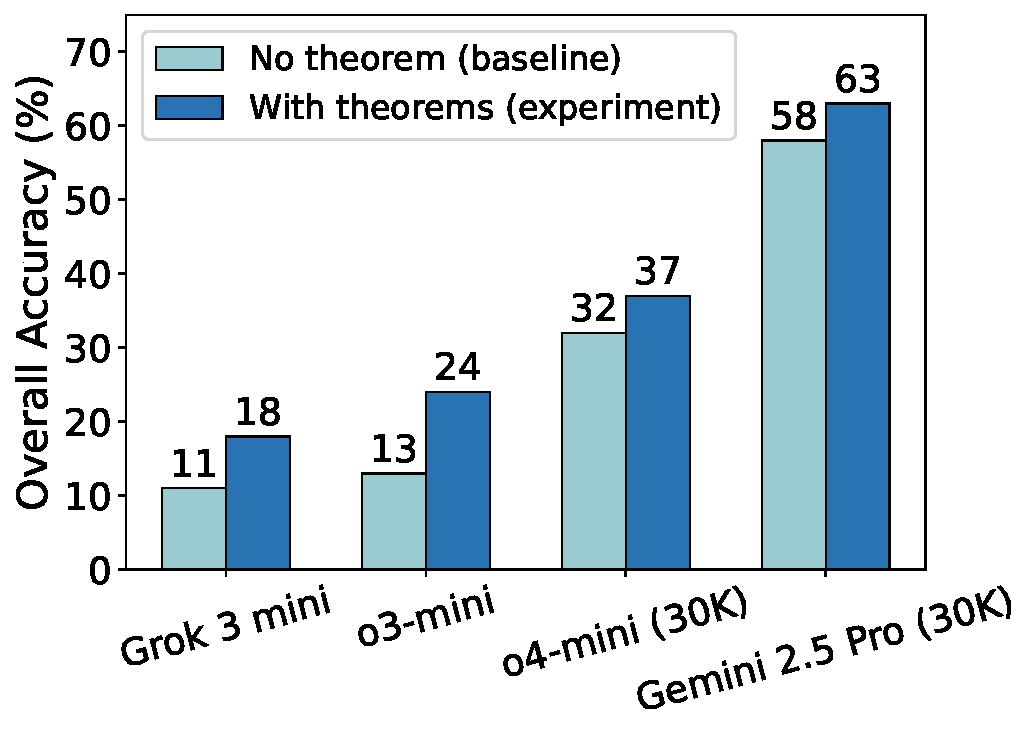
\includegraphics[width=1.0\linewidth]{figs/explore_theorem_as_hint_overall_acc.pdf}
        \caption{Model performance with annotated theorems as hints (\textit{Overall Accuracy}).}
        \label{fig:explore_theorem_as_hint_overall_acc}
    \end{minipage}
    \hfill
    \begin{minipage}{0.49\textwidth}
        \centering
        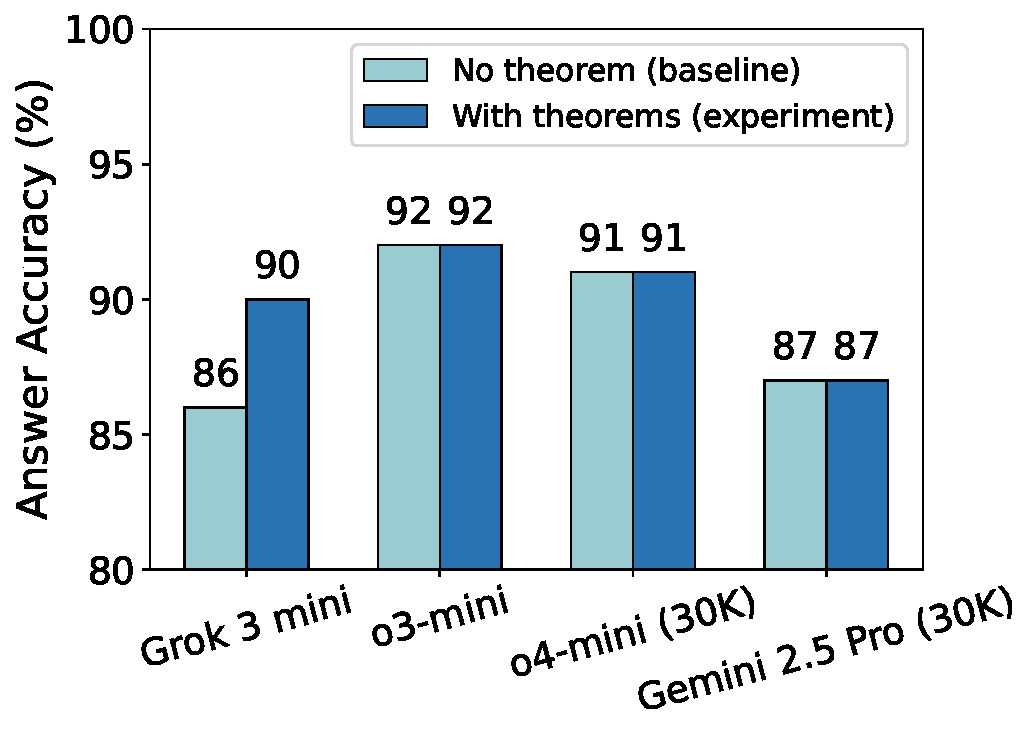
\includegraphics[width=1.0\linewidth]{figs/explore_theorem_as_hint_answer_acc.pdf}
        \caption{Model performance when taking annotated theorems as hints (\textit{Answer Accuracy}).}
        \label{fig:explore_theorem_as_hint_answer_acc}
    \end{minipage}
    \vspace{-3mm}
\end{figure}


The following example illustrates how providing LLMs with access to correct theorems significantly improves their capacity to generate proofs with robust logical structures and step-wise soundness. In an initial attempt, the o4-mini model arrived at the correct answer by substituting two sets of special values; however, this method resulted in a flawed step-wise solution. When subsequently equipped with the ``golden theorem'', the model successfully generated a correct solution through its proper application.

\begin{examplebox}[Taking Annotated Theorems as Hints: Example]
\textbf{Problem:} Let $a, b, c$ be the lengths of the sides of a triangle, such that $a + b + c = 3$. Determine the largest constant $C$ such that the following inequality holds for all $a, b, c$:
$$
a^{2} + b^{2} + c^{2} + \frac{4 a b c}{3} \geq C.
$$
\\
\textbf{Related Theorem:}\\ 
\correct{\textbf{Theorem Zdravko (Mean inequalities)}}: Let $a_{1}, a_{2}, \ldots, a_{n}$ be positive real numbers. The numbers
$$
\begin{aligned}
& Q M=\sqrt{\frac{a_{1}^{2}+a_{2}^{2}+\cdots+a_{n}^{2}}{n}}, \quad A M=\frac{a_{1}+a_{2}+\cdots+a_{n}}{n} \\
& G M=\sqrt[n]{a_{1} a_{2} \cdots a_{n}} \quad \text { and } \quad H M=\frac{n}{\frac{1}{a_{1}}+\frac{1}{a_{2}}+\cdots+\frac{1}{a_{n}}}
\end{aligned}
$$
are called the quadratic, arithmetic, geometric and harmonic mean for the numbers $a_{1}, a_{2}, \ldots, a_{n}$, respectively, and we have
$$
\correct{Q M \geq A M \geq G M \geq H M}
$$

Equalities occur if and only if $a_{1}=a_{2}=\cdots=a_{n}$.
\\\\
\textbf{Response by o4-mini without any Theorem Hint (Incorrect Response \xmark):}\\
Let $F(a, b, c) = a^2 + b^2 + c^2 + \frac{4}{3}abc$.\\
\wrong{\textbf{1. Equilateral case:} Let \( a = b = c = 1 \)}. Then \( a + b + c = 3 \), and
\[
F(1,1,1) = 1^2 + 1^2 + 1^2 + \frac{4}{3} \cdot 1 \cdot 1 \cdot 1 = 3 + \frac{4}{3} = \frac{13}{3}
\]

\wrong{\textbf{2. Degenerate case:} Let  \( a = b = 0.75,\ c = 1.5 \)}. Then,
\[
F(0.75, 0.75, 1.5) = 0.75^2 + 0.75^2 + 1.5^2 + \frac{4}{3} \cdot 0.75 \cdot 0.75 \cdot 1.5 = 4.5
\]

Thus, on the boundary we have \( F(a,b,c) \geq 4.5 \).\\

\wrong{A more detailed check of the two-equal-sides slice \( a = b = x,\ c = 3 - 2x \) shows that} \( F(x) \) attains its unique minimum \( 13/3 \) at \( x = 1 \). No other interior configuration yields a smaller value. Therefore, the answer is \boxed{C = \frac{13}{3}}.
\\

% \textbf{(Continued)}

% \end{examplebox}

% \begin{examplebox}[Taking Annotated Theorems as Hints: Example (Continued)]

\textbf{Response by o4-mini with a Theorem Hint (Correct Response \cmark):}
Set \(a+b+c=3\).  \correct{By the quadratic–arithmetic mean inequality (QM–AM) in \textbf{Mean inequalities theorem}},
\[
\frac{a^2+b^2+c^2}{3}\ge\Bigl(\frac{a+b+c}{3}\Bigr)^2=1
\quad\Longrightarrow\quad
a^2+b^2+c^2\ge3.
\]
\correct{By the AM–GM inequality in \textbf{Mean inequalities theorem}},
\[
\sqrt[3]{abc}\le\frac{a+b+c}{3}=1
\quad\Longrightarrow\quad
abc\le1.
\]
Hence
\[
a^2+b^2+c^2+\frac{4abc}{3}
\;\ge\;3+\frac{4\cdot1}{3}
\;=\;3+\frac43
\;=\;\frac{13}{3}.
\]
Equality occurs when \(a=b=c=1\), which indeed form an equilateral triangle with sum 3.  Thus the largest constant \(C\) for which the inequality holds for all triangles is
\[
C=\frac{13}{3}.
\]
The answer is \boxed{C=13/3}.
\\\\
\textbf{Expert Comment:} 
In the version without the theorem, the model relies on toy-case evaluations—specifically symmetric and degenerate configurations—to guess the correct bound \wronghl. In addition, its reasoning includes a clear logical gap: it claims that “a more detailed check of the two-equal-sides slice $a = b = x,\ c = 3 - 2x$” shows the minimum occurs at $x = 1$, but provides no explanation or computation to support this claim \wronghl. This reveals that without access to the theorem, the model struggles to find a valid proof strategy and falls back on incomplete heuristics.
\\\\
Once the relevant inequality theorems are provided, the model quickly applies the QM–AM and AM–GM inequalities from the \correct{\textbf{Mean inequalities theorem}} correctly \correcthl. It uses these tools to derive a general lower bound valid for all triangles, leading rigorously to the correct constant $C = \frac{13}{3}$. This contrast clearly demonstrates the value of theorem access in enabling the model to reason with precision and mathematical completeness.

\end{examplebox}

% \clearpage
\subsubsection{Retrieval as Augmentation}
\label{app:explore_retrieve_relevant_theorem_as_hints}

\subparagraph{Retrieving relevant theorems as hints.} 
We also evaluate the impact of theorem-based hints on answer accuracy. This evaluation was conducted on the same 40-problem subset used in the main experiments, with models receiving the top-$k$ most frequent theorems from the \dataset training set as hints. As shown in Figure~\ref{fig:explore_frequent_theorem_as_hints_answer_acc}, providing one or two retrieved theorems tends to reduce \textit{final-answer} accuracy for weaker models, such as Grok 3 mini and o3-mini. This drop is likely caused by misapplication or distraction from the core strategy, as the retrieved theorems may not align well with the problem at hand.

\begin{figure}[th!]
    \centering
    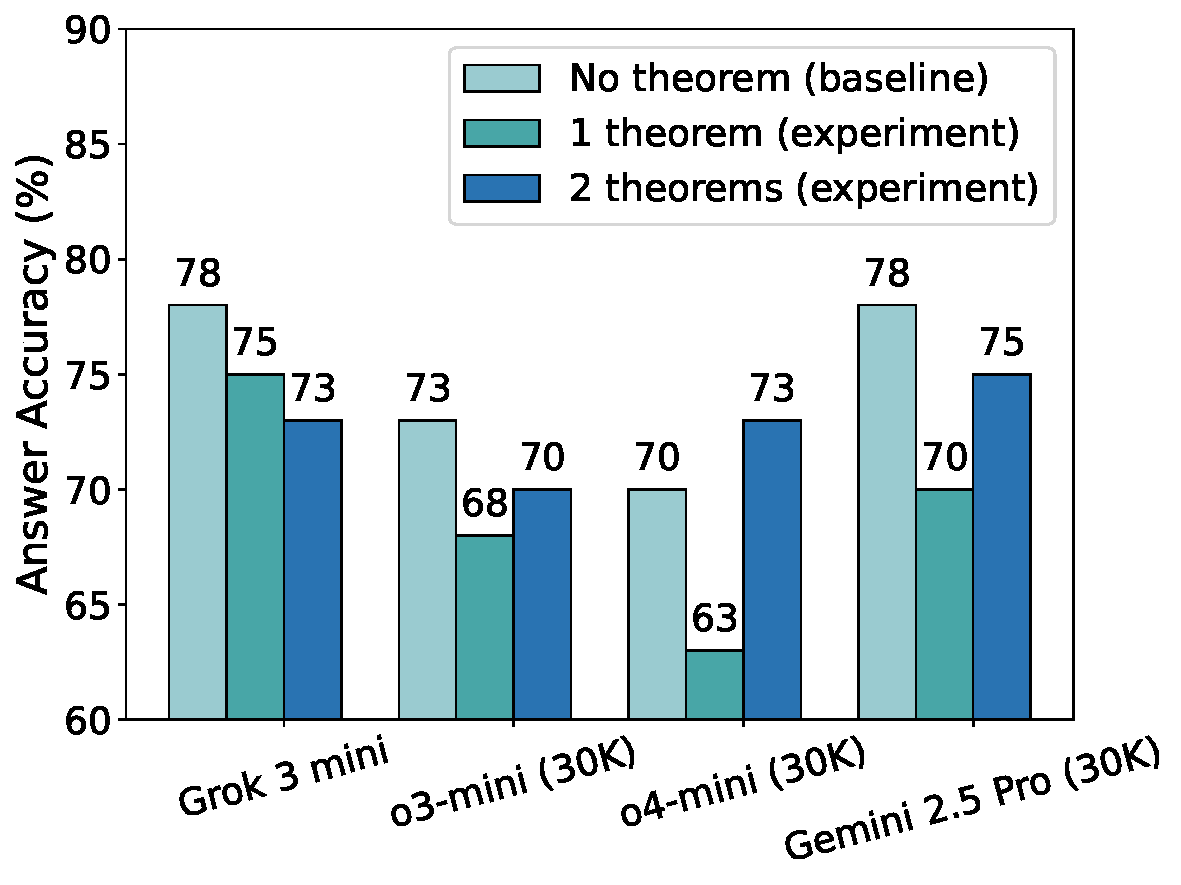
\includegraphics[width=0.55\linewidth]{figs/explore_frequent_theorem_as_hints_answer_acc.pdf}
    \caption{Model performance when taking most frequent theorems as hints (\textit{Answer Accuracy}).}
    \label{fig:explore_frequent_theorem_as_hints_answer_acc}
\end{figure}

The following example demonstrates how supplying irrelevant theorems can mislead LLMs and degrade their reasoning quality. Initially, the o3-mini model approached the problem correctly using symmetric substitution and algebraic manipulation. However, after being provided with the Mean Inequality theorem—unrelated to the actual solution—it abandoned its structured strategy and instead attempted to apply the AM–GM in Mean inequalities directly, without proper justification. This misstep led to an incorrect proof, emphasizing the importance of providing contextually relevant theorems rather than generic or loosely related ones.

\begin{examplebox}[Retrieving Relevant Theorems as Hints: Example]
\small
\textbf{Problem:} Let $a, b, c$ be positive real numbers. Consider the following inequality:
$$
\sum_{cyc} \frac{b+c}{\sqrt{(a+b)(a+c)}} \quad () \quad 2 \sum_{cyc} \frac{2a}{2b+c}.
$$
Determine the correct inequality relation to fill in the blank.\\
\textbf{Options:} (A) $\leq$ \quad(B) $\geq$ \quad (C) $=$  \quad (D) $<$ \quad  (E) $>$  \quad (F) None of the above
\\\\
\textbf{Response by o4-mini without Theorems (Correct Response \cmark):}

First note the elementary two‐term bound, valid for all positive \(u,v\):
\[
\frac{2u}{2v+w}+\frac{2u}{2w+v}
\;-\;\frac{v+w}{\sqrt{(u+v)(u+w)}}
\;=\;\frac{\bigl(\sqrt{(u+v)(u+w)}-u\bigr)^2}{\sqrt{(u+v)(u+w)}\,(2v+w)(2w+v)}
\;>\;0.
\]
If expanding and simplifying that difference you arrive precisely at
\[
\frac{v+w}{\sqrt{(u+v)(u+w)}}\;<\;
\frac{2u}{2v+w}+\frac{2u}{2w+v}.
\]
Now set \((u,v,w)=(a,b,c)\), and sum the resulting three inequalities cyclically.  

On the right you get $\sum_{\rm cyc}\!\Bigl[\frac{2a}{2b+c}+\frac{2a}{2c+b}\Bigr]
=\;2\sum_{\rm cyc}\frac{2a}{2b+c}$. 
While on the left you recover \(\sum_{\rm cyc}\tfrac{b+c}{\sqrt{(a+b)(a+c)}}\).  Thus in full generality
\[
\sum_{\rm cyc}\frac{b+c}{\sqrt{(a+b)(a+c)}}\;<\;
2\sum_{\rm cyc}\frac{2a}{2b+c},
\]
Therefore, the answer is \boxed{(D) <}
\\\\
\textbf{Irrelevant Theorem Provided:} \textbf{Theorem Zdravko (Mean Inequalities)}: Let $a_{1}, a_{2}, \ldots, a_{n}$ be positive real numbers. The numbers
$$
\begin{aligned}
& Q M=\sqrt{\frac{a_{1}^{2}+a_{2}^{2}+\cdots+a_{n}^{2}}{n}}, \quad A M=\frac{a_{1}+a_{2}+\cdots+a_{n}}{n} \\
& G M=\sqrt[n]{a_{1} a_{2} \cdots a_{n}} \quad \text { and } \quad H M=\frac{n}{\frac{1}{a_{1}}+\frac{1}{a_{2}}+\cdots+\frac{1}{a_{n}}}
\end{aligned}
$$
are called the quadratic, arithmetic, geometric and harmonic mean for the numbers $a_{1}, a_{2}, \ldots, a_{n}$, respectively, and we have
$$
Q M \geq A M \geq G M \geq H M
$$

Equalities occur if and only if $a_{1}=a_{2}=\cdots=a_{n}$.
\\\\
\textbf{Response by o4-mini with Theorem Provided (Incorrect Response \xmark):}

First, when \(a=b=c=1\), we have
\[LHS 
= \sum_{\rm cyc}\frac{b+c}{\sqrt{(a+b)(a+c)}}
=3,\quad
RHS 
= 2\sum_{\rm cyc}\frac{2a}{2b+c} =4.
\]

Hence at \(a=b=c\), 
\[
LHS = 3 < RHS = 4.
\]
\wrong{A more detailed inequality‐chasing via AM–GM in Mean inequalities theorem shows the strict “<” persists for all positive \(a,b,c\).}

Therefore, the answer is \boxed{(D) <} 
\\\\
\textbf{Expert Comment:}
Without theorems, the model solves the problem accurately by constructing a detailed inequality using symmetric substitution and algebraic manipulation. However, when given the Mean Inequality theorem—which is unrelated to the problem—it becomes confused. Instead of following the previous structured reasoning, it resorts to a surface-level AM–GM (Mean inequalities) without general proof or justification \wronghl. This highlights the importance of supplying relevant theorems.
\end{examplebox}

\subparagraph{Retrieving training problems as demonstrations.} 
Building on our observation that providing relevant theorems can enhance performance in inequality reasoning (\S\ref{sec:improvement_strategies}, \S\ref{app:explore_theorem_as_hints_appendix}, \S\ref{app:explore_retrieve_relevant_theorem_as_hints}), we now investigate whether using training problems with step-wise solutions as demonstrations is similarly beneficial. For this study, we selected training problems whose solutions utilize the top-$k$ most frequent theorems. As shown by the overall accuracy in Figure~\ref{fig:explore_frequent_solutions_as_hints_overall_acc}, Grok 3 mini's performance improves from a baseline of 10\% (with no demonstration problem) to 13\% when provided with one such problem. However, its accuracy drops sharply to 3\% when two problems are used as demonstrations. Similarly, Gemini 2.5 Pro peaks at 53\% accuracy with one demonstration problem, declining to 45\% with two. o4-mini reaches 23\% accuracy with one demonstration problem, a 3\% increase from its 20\% baseline (without demonstrations). 

The answer accuracy, presented in Figure~\ref{fig:explore_frequent_solutions_as_hints_answer_acc}, exhibits similar instability. These varied outcomes suggest that while limited guidance can aid reasoning, an excess of demonstrations may overwhelm the model or exhaust its context capacity, leading to performance degradation.

\begin{figure}[H]
    \centering
    \begin{minipage}{0.485\textwidth}
        \centering
        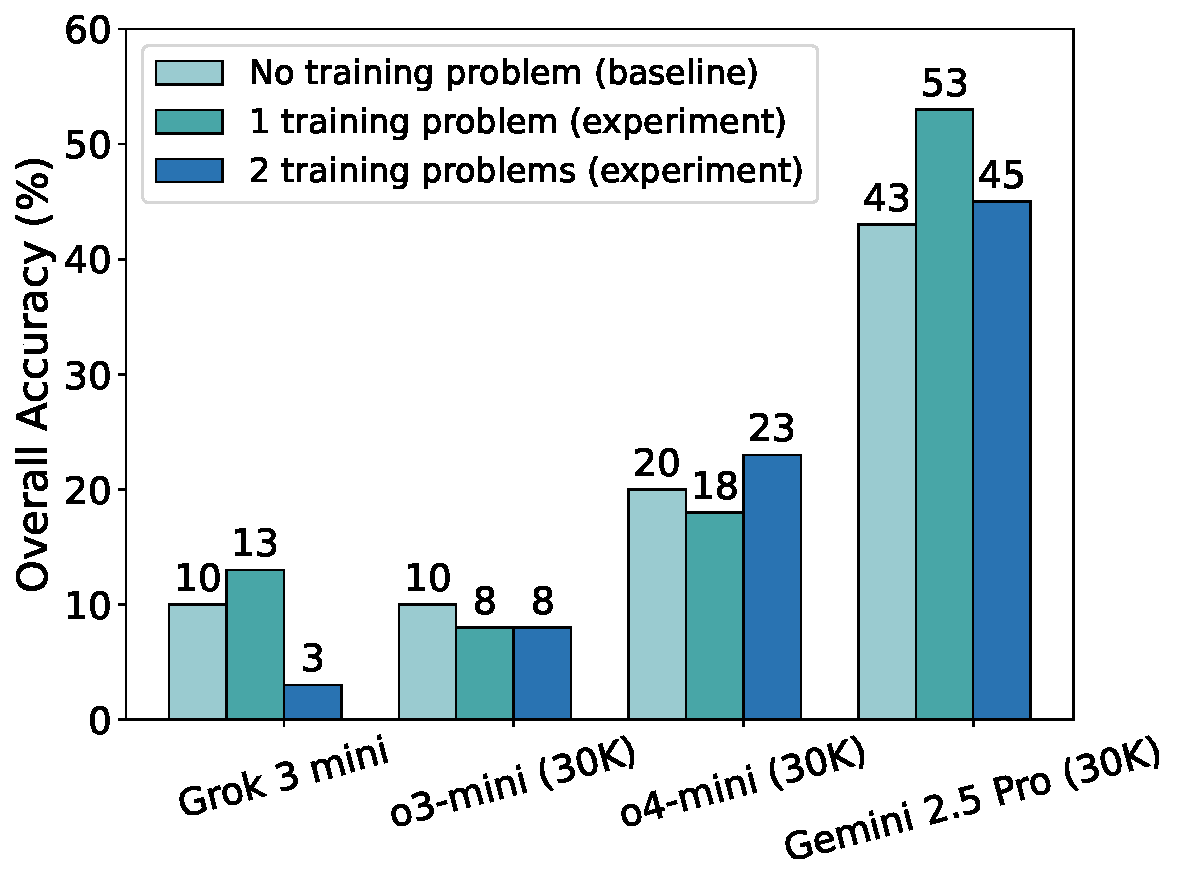
\includegraphics[width=1.0\linewidth]{figs/explore_frequent_solutions_as_hints_overall_acc.pdf}
        \caption{Model performance when taking example solutions associated with the top-$k$ frequent theorems as hints (\textit{Overall Accuracy}).}
        \label{fig:explore_frequent_solutions_as_hints_overall_acc}
    \end{minipage}
    \hfill
    \begin{minipage}{0.485\textwidth}
        \centering
        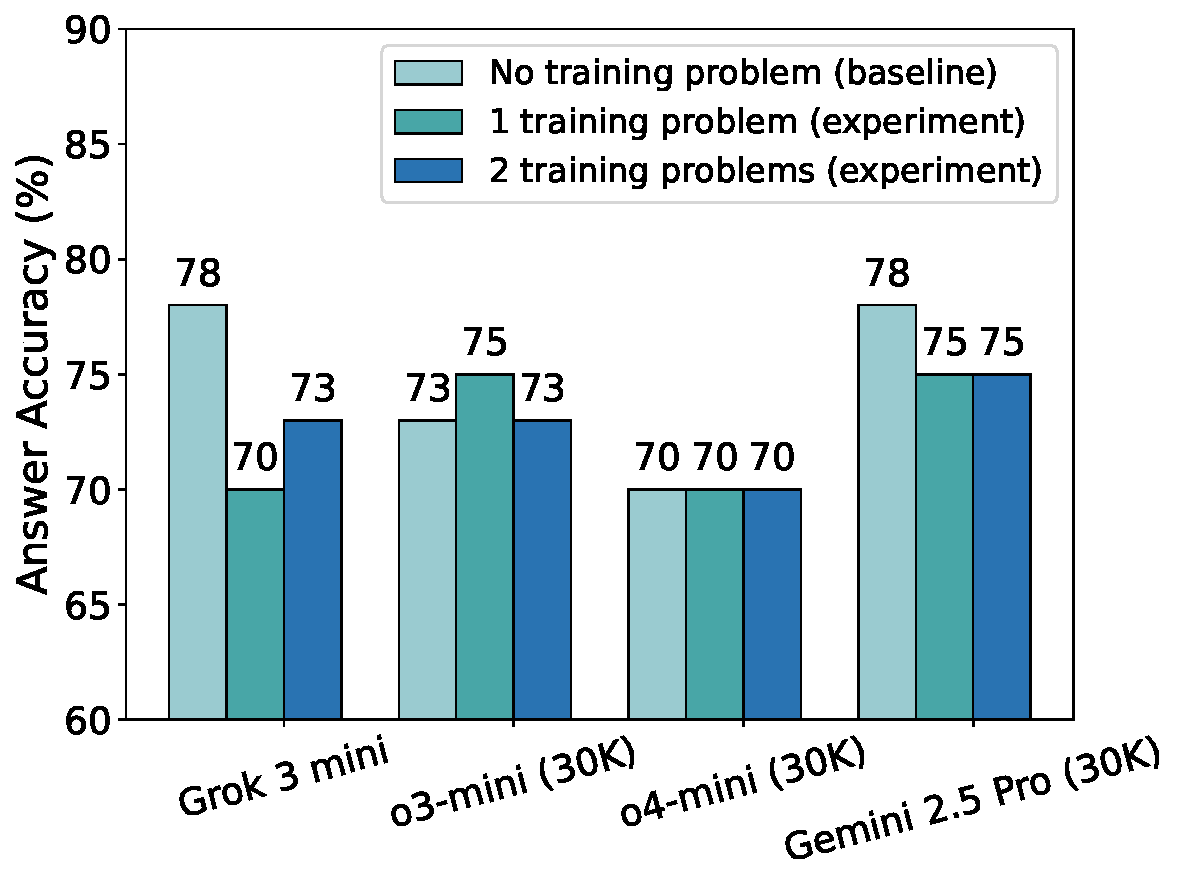
\includegraphics[width=1.0\linewidth]{figs/explore_frequent_solutions_as_hints_answer_acc.pdf}
        \caption{Model performance when taking example solutions associated with the top-$k$ frequent theorems as hints (\textit{Answer Accuracy}).}
        \label{fig:explore_frequent_solutions_as_hints_answer_acc}
    \end{minipage}
    \vspace{-3mm}
\end{figure}


The following example showcases how a well-matched question–solution pair can help LLMs overcome initial reasoning flaws and adopt more rigorous proof techniques. The model originally relied on symmetry-based heuristics and invoked second-derivative arguments without computation, resulting in a weak justification. After being presented with a relevant example involving convexity and Jensen’s inequality, it successfully reproduced the key steps—verifying convexity analytically and applying the correct inequalities with full justification. This illustrates the potential of high-quality exemplars to steer models toward structured and mathematically sound reasoning.


\begin{examplebox}[Retrieving Training Problems as Demonstrations: Example]
\textbf{Question:} Let $a, b > 0$ such that $a + b = 1$. Determine the largest constant $C$ such that the following inequality holds for all $a, b$:
$$
\left(a+\frac{1}{a}\right)^2+\left(b+\frac{1}{b}\right)^2 \geq C.
$$
\\
\textbf{Ground Truth:} \boxed{C = \frac{25}{2}}
\\\\
\textbf{Response by o4-mini without Examples (Incorrect Response \xmark)}:

Define
$
f(a) = \left(a + \frac{1}{a} \right)^2 + \left((1 - a) + \frac{1}{1 - a} \right)^2, \quad 0 < a < 1.
$

1. \wrong{The function \( f \) is symmetric about \( a = \frac{1}{2} \). Hence any interior extremum must occur at \( a = \frac{1}{2} \).}

2. At \( a = \frac{1}{2} \), we have
    $
    f\left(\frac{1}{2}\right) = 2 \cdot \frac{25}{4} = \frac{25}{2}.
    $

3. \wrong{Checking the second derivative shows this is indeed a minimum.} The answer is \boxed{ C = \frac{25}{2} }.
\\\\
\textbf{Example Questions:}Let $a, b, c$ be positive real numbers such that $a^2 + b^2 + c^2 = 3abc$. Find the largest constant $C$ such that the following inequality holds for all $a, b, c$ satisfying the given constraint:
$$
\frac{a}{b^2 c^2} + \frac{b}{c^2 a^2} + \frac{c}{a^2 b^2} \geq \frac{C}{a+b+c}
$$
\textbf{Example Solution:} The given inequality is equivalent to$$\left(a^{3}+b^{3}+c^{3}\right)(a+b+c) \geq 9 a^{2} b^{2} c^{2}$$Applying the Cauchy-Schwarz inequality we have$$\left(a^{3}+b^{3}+c^{3}\right)(a+b+c) \geq\left(a^{2}+b^{2}+c^{2}\right)^{2}$$Since $a^{2}+b^{2}+c^{2}=3 a b c$ we obtain$$\left(a^{3}+b^{3}+c^{3}\right)(a+b+c) \geq\left(a^{2}+b^{2}+c^{2}\right)^{2}=(3 a b c)^{2}=9 a^{2} b^{2} c^{2}$$Equality holds if and only if $a=b=c=1$.
Therefore, the answer is \boxed{C = 9}.
\\\\
\textbf{Response by o4-mini with Examples (Correct Response \cmark):}
Let \(a,b>0\) with \(a+b=1\).  Define the function
$
f(a)\;=\;\Bigl(a+\tfrac1a\Bigr)^2\;+\;\Bigl(b+\tfrac1b\Bigr)^2
,\quad b=1-a.
$\\
Convexity argument: consider the function 
    $h(x)=\Bigl(x+\tfrac1x\Bigr)^2\quad(x>0).$ 
    
\correct{Compute its second derivative: $ h(x)=x^2+2+\tfrac1{x^2}, \quad h''(x)=2+6x^{-4}>0,\quad\forall x>0$}

    \correct{Hence \(h\) is convex on \((0,\infty)\).}  Since \(a\) and \(b\) satisfy \(a+b=1\), by \textcolor{blue}{Jensen’s inequality for the convex function \(h\) we have}
    \[
      \frac{h(a)+h(b)}2
      \;\ge\;
      h\!\Bigl(\tfrac{a+b}2\Bigr)
      =h\!\Bigl(\tfrac12\Bigr)
      =\Bigl(\tfrac12+2\Bigr)^2
      =\Bigl(\tfrac52\Bigr)^2
      =\frac{25}4.
    \]
    Therefore$f(a)=h(a)+h(b)\;\ge\;2\cdot\frac{25}4=\frac{25}{2}.$, i.e. The answer is \boxed{C=\frac{25}{2}}.

\textbf{Expert Comment:} The initial solution lacks rigor: it incorrectly assumes that symmetry implies a unique minimum, and references the second derivative without computing it \wronghl. However, after being provided with a related example that uses a careful convexity argument and the Cauchy-Schwarz inequality, the model is able to imitate the correct reasoning. It verifies convexity via the second derivative, correctly applies Jensen’s inequality, and explicitly justifies the minimum \correcthl. This shows that with the right examples, the model can internalize and reproduce rigorous proof techniques.
\end{examplebox}



% \clearpage
\subsubsection{Self-improvement via Critic as Feedback}
\label{app:self_improvement}
In addition to overall accuracy, we also evaluate answer accuracy within the same self-critique setup. Using 40 randomly selected problems from the \dataset benchmark, we assess whether one round of self-revision improves the correctness of final answers. As shown in Figure~\ref{fig:explore_self_critic_as_hint_answer_acc}, models like o3-mini and o4-mini gain 2–5\% in answer accuracy after revision. This result further supports self-critique as a lightweight and supervision-free approach to improving solution reliability in inequality problems.
\begin{figure}[H]
    \centering
    \vspace{-2mm}
    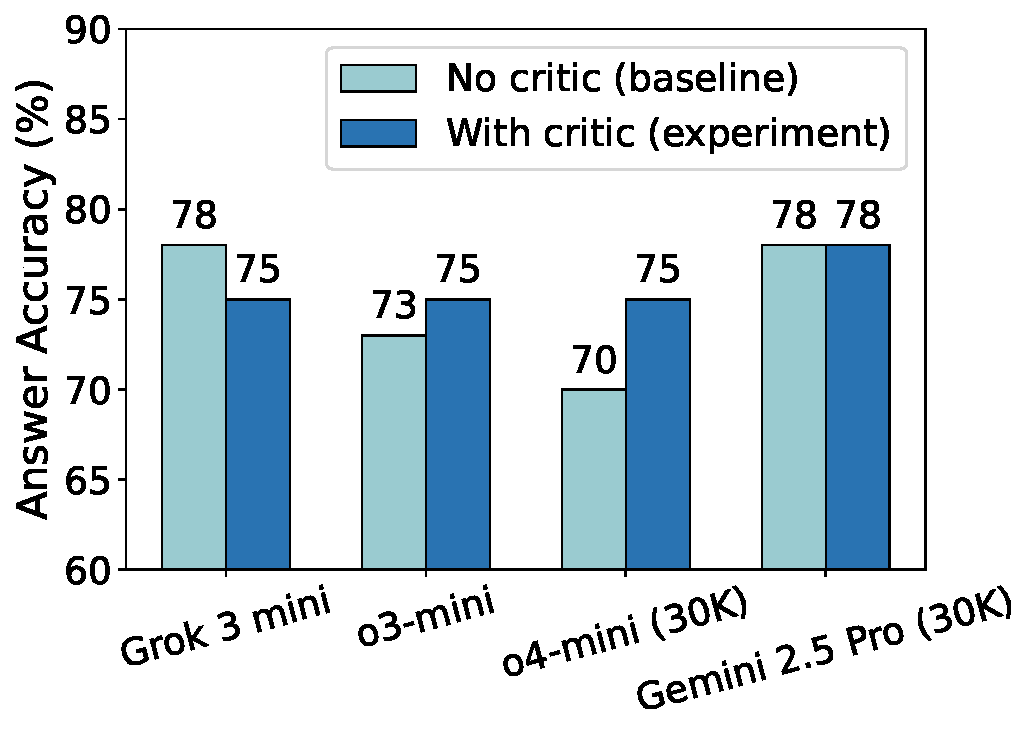
\includegraphics[width=0.45\linewidth]{figs/explore_self_critic_as_hint_answer_acc.pdf}
    \caption{Model performance when taking one round of critic as feedback (\textit{Answer Accuracy}).}
    \vspace{-4mm}
\label{fig:explore_self_critic_as_hint_answer_acc}
\end{figure}

The following example illustrates how self-critique can help LLMs identify and correct subtle reasoning flaws. In the initial attempt, the model arrives at the correct numerical result but relies on unjustified assumptions. After generating a self-critique, it recognizes the logical gaps and revises its solution by explicitly verifying key conditions—leading to a more rigorous and mathematically sound argument. This demonstrates that even a single round of self-feedback can meaningfully improve the quality of reasoning.

\begin{examplebox}[Self-improvement via Critic as Feedback: Example]
\textbf{Problem}: Let $a, b > 0$ such that $a + b = 1$. Determine the largest constant $C$ such that the following inequality holds for all $a, b$:
$$
\left(a+\frac{1}{a}\right)^2+\left(b+\frac{1}{b}\right)^2 \geq C.
$$

\textbf{Ground Truth:} \boxed{C = \frac{25}{2}}


\textbf{Initial Response by o4-mini (Incorrect Response \xmark):}\\
Define
$
f(a) = \left(a + \frac{1}{a} \right)^2 + \left((1 - a) + \frac{1}{1 - a} \right)^2, \quad 0 < a < 1.
$

1. \wrong{The function \( f \) is symmetric about \( a = \frac{1}{2} \). Hence any interior extremum must occur at \( a = \frac{1}{2} \).}

2. At \( a = \frac{1}{2} \), we have
    $
    f\left(\frac{1}{2}\right) = 2 \cdot \frac{25}{4} = \frac{25}{2}.
    $

3. \wrong{Checking the second derivative shows this is indeed a minimum.} The answer is \boxed{ C = \frac{25}{2} }.

\textbf{Self-critic Feedback by o4-mini}:

These are what make this solution incompletely justified:

\begin{itemize}
    \item symmetry alone guarantees \( f'(1/2) = 0 \), but it does \emph{not} by itself rule out other critical points \( a \ne 1/2 \). In general, a symmetric \( C^1 \)-function can have multiple stationary points symmetrically placed about the center. 
    
    \item You assert ``checking the second derivative shows this is indeed a minimum,'' but you never exhibit \( f''(1/2) \) or argue it is positive. 
\end{itemize}
$\quad$\\
\textbf{Refined Solution by o4-mini (Correct Response \cmark):} \\Define the function
$
f(a) = \left(a + \frac{1}{a} \right)^2 + \left((1 - a) + \frac{1}{1 - a} \right)^2,
$
for \( a \in (0,1) \). Let \( g(x) = \left(x + \frac{1}{x} \right)^2 \) for \( x > 0 \). Then \( f(a) = g(a) + g(1 - a) \).
\\
\\
Compute:

\[
g(x) = x^2 + 2 + \frac{1}{x^2}, \quad g'(x) = 2x - \frac{2}{x^3}, \quad g''(x) = 2 + \frac{6}{x^4} > 0.
\]
Hence, \( g \) is strictly convex on \( (0, \infty) \).
\\\\
Since \( f''(a) = g''(a) + g''(1 - a) \) and each term is positive for \( a \in (0,1) \), \correct{we have \( f''(a) > 0 \). Thus, \( f \) is strictly convex on \( (0,1) \)}
A strictly convex \( C^1 \)-function on an open interval has at most one critical point, which, if it exists, is its global minimum. We compute:
\[\correct{
f'(a) = g'(a) - g'(1 - a)=0}
\]

\correct{By symmetry, we can solve it and get \( a = \frac{1}{2} \)}. Hence the unique solution of \( f'(a) = 0 \) in \( (0,1) \) is \( a = \frac{1}{2} \).

Therefore, the smallest possible value is  \boxed{C=f\left(\frac{1}{2} \right) = \frac{25}{2}}.
\\\\
\textbf{Expert Comment:}
The initial solution gets the correct value $C = \frac{25}{2}$, but lacks rigor: it incorrectly assumes that symmetry implies a unique minimum, and references the second derivative without computing it \wronghl. The critic accurately points out these gaps. The refined solution corrects them by proving convexity through second derivatives and confirming $a = \frac{1}{2}$ is the unique minimizer through first derivatives \correcthl. This demonstrates that self-criticism effectively improves the mathematical soundness of the argument.

\end{examplebox}


% \clearpage
\subsubsection{Few-shot Evaluation} % Few-shot evaluation
\label{app:few_shot_evaluation}

We also investigated the effect of few-shot prompting on the \dataset test set. Specifically, we compared zero-shot, one-shot, and three-shot configurations across different models. 

As shown in Figure~\ref{fig:few_shot_overall_acc}, the gains in overall accuracy from few-shot prompting were small, typically below 2\% compared to zero-shot performance. For instance, Grok 3 achieved 3.5\% accuracy in the zero-shot setting but dropped slightly in the one-shot and three-shot settings (2.5\% and 1.5\%, respectively). Similarly, o1 peaked at 8.0\% in both the one-shot and three-shot settings, with minimal difference across shots.

\begin{figure}[H]
    \centering
    \begin{minipage}{0.485\textwidth}
        \centering
        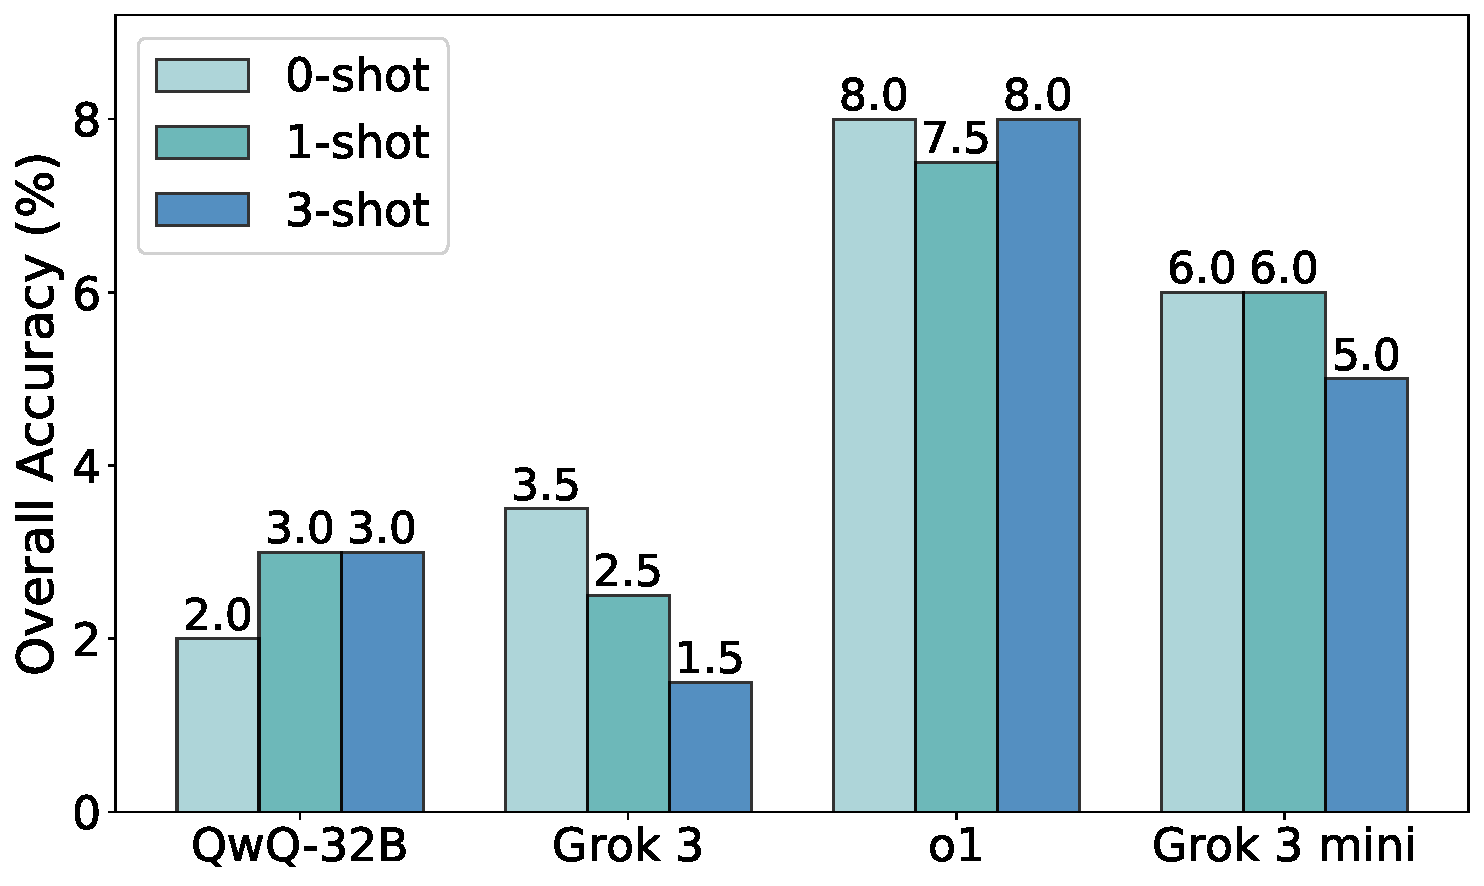
\includegraphics[width=1.0\linewidth]{figs/few_shot_overall_acc_figure.pdf}
        \caption{Model performance under zero-shot, one-shot, and three-shot settings (\textit{Overall Accuracy}).}
        \label{fig:few_shot_overall_acc}
    \end{minipage}
    \hfill
    \begin{minipage}{0.485\textwidth}
        \centering
        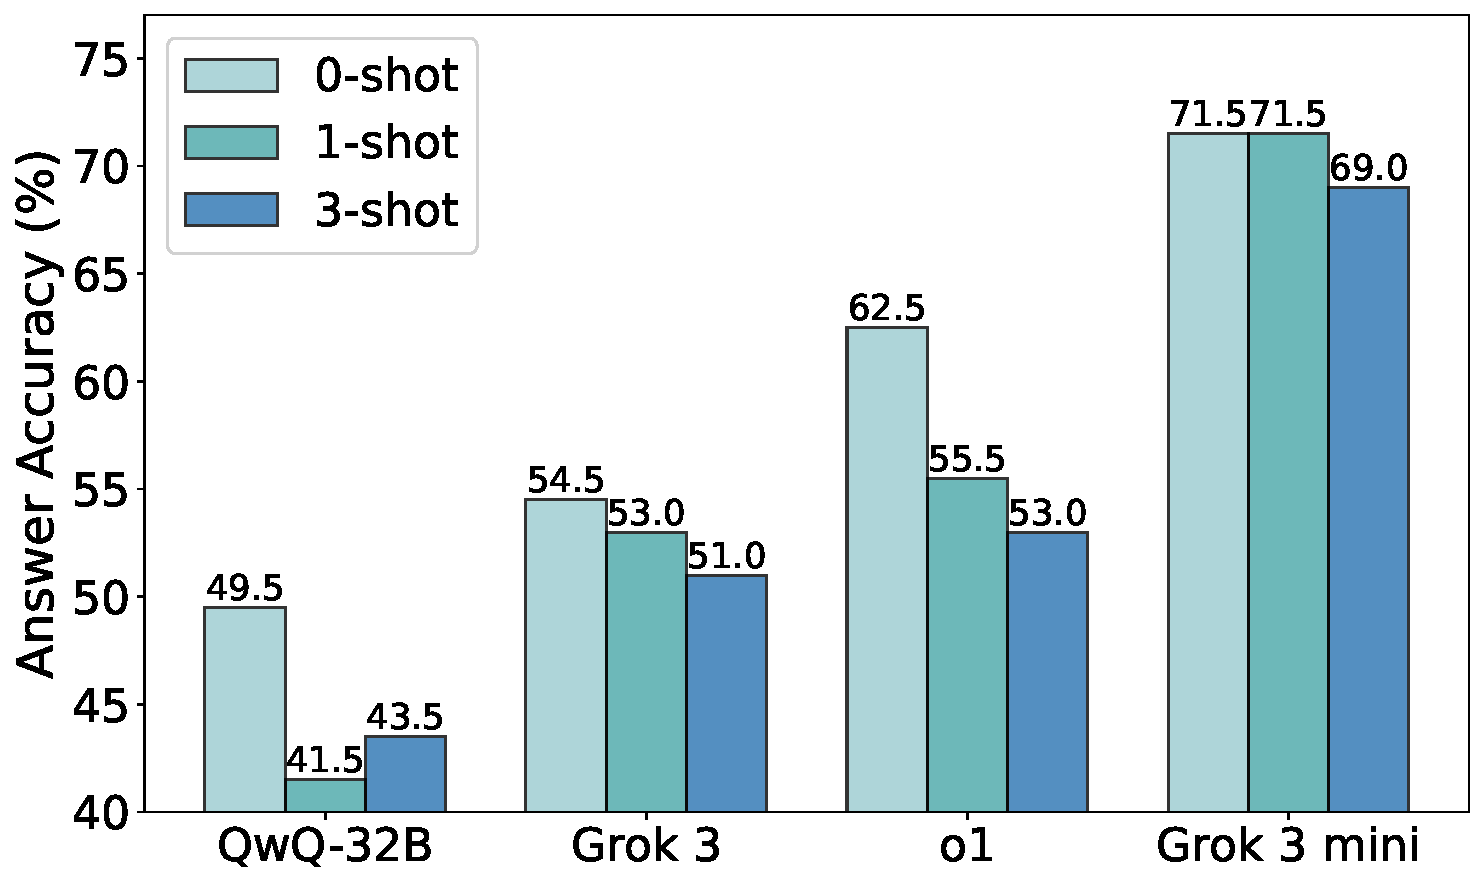
\includegraphics[width=1.0\linewidth]{figs/few_shot_answer_acc_figure.pdf}
        \caption{Model performance under zero-shot, one-shot, and three-shot settings (\textit{Answer Accuracy}).}
        \label{fig:few_shot_answer_acc}
    \end{minipage}
    \vspace{-3mm}
\end{figure}

Moreover, Figure~\ref{fig:few_shot_answer_acc} shows that few-shot prompting typically reduces answer accuracy. For o1, accuracy drops from 62.5\% in the zero-shot setting to 55.5\% with one-shot and 53.0\% with three-shot. QwQ-32B displays the same trend: both one-shot and three-shot underperform the zero-shot baseline (41.5\% and 43.5\% vs.\ 49.5\%). These declines suggest overfitting to exemplars, indicating that few-shot prompting does not reliably improve the answer accuracy on the \dataset test set.


% \clearpage
\subsubsection{Evaluation on the Formalized \dataset}
\label{app:formal_evaluation}

To expand the impact of \dataset, we conduct a formal evaluation on state-of-the-art automated theorem proving (ATP) models. The key step in this evaluation is the \textbf{formalization process}, which converts the natural language inequality problems in \dataset into machine-verifiable Lean4 code. 

As illustrated in Figures~\ref{fig:formal_illustration_bound} and Figures~\ref{fig:formal_illustration_relation}, this process proceeds in two stages in our experiment. First, we reformulate the inequality problems into proof-style problems using GPT-4.1~\cite{openai2025gpt41}, ensuring they are structured for formalization. Second, we employ the Goedel-Formalizer-V2-32B~\cite{lin2025goedelv2} to automatically translate these reformulated proof problems into valid Lean4 representations.

\begin{figure}[H]
    \centering
    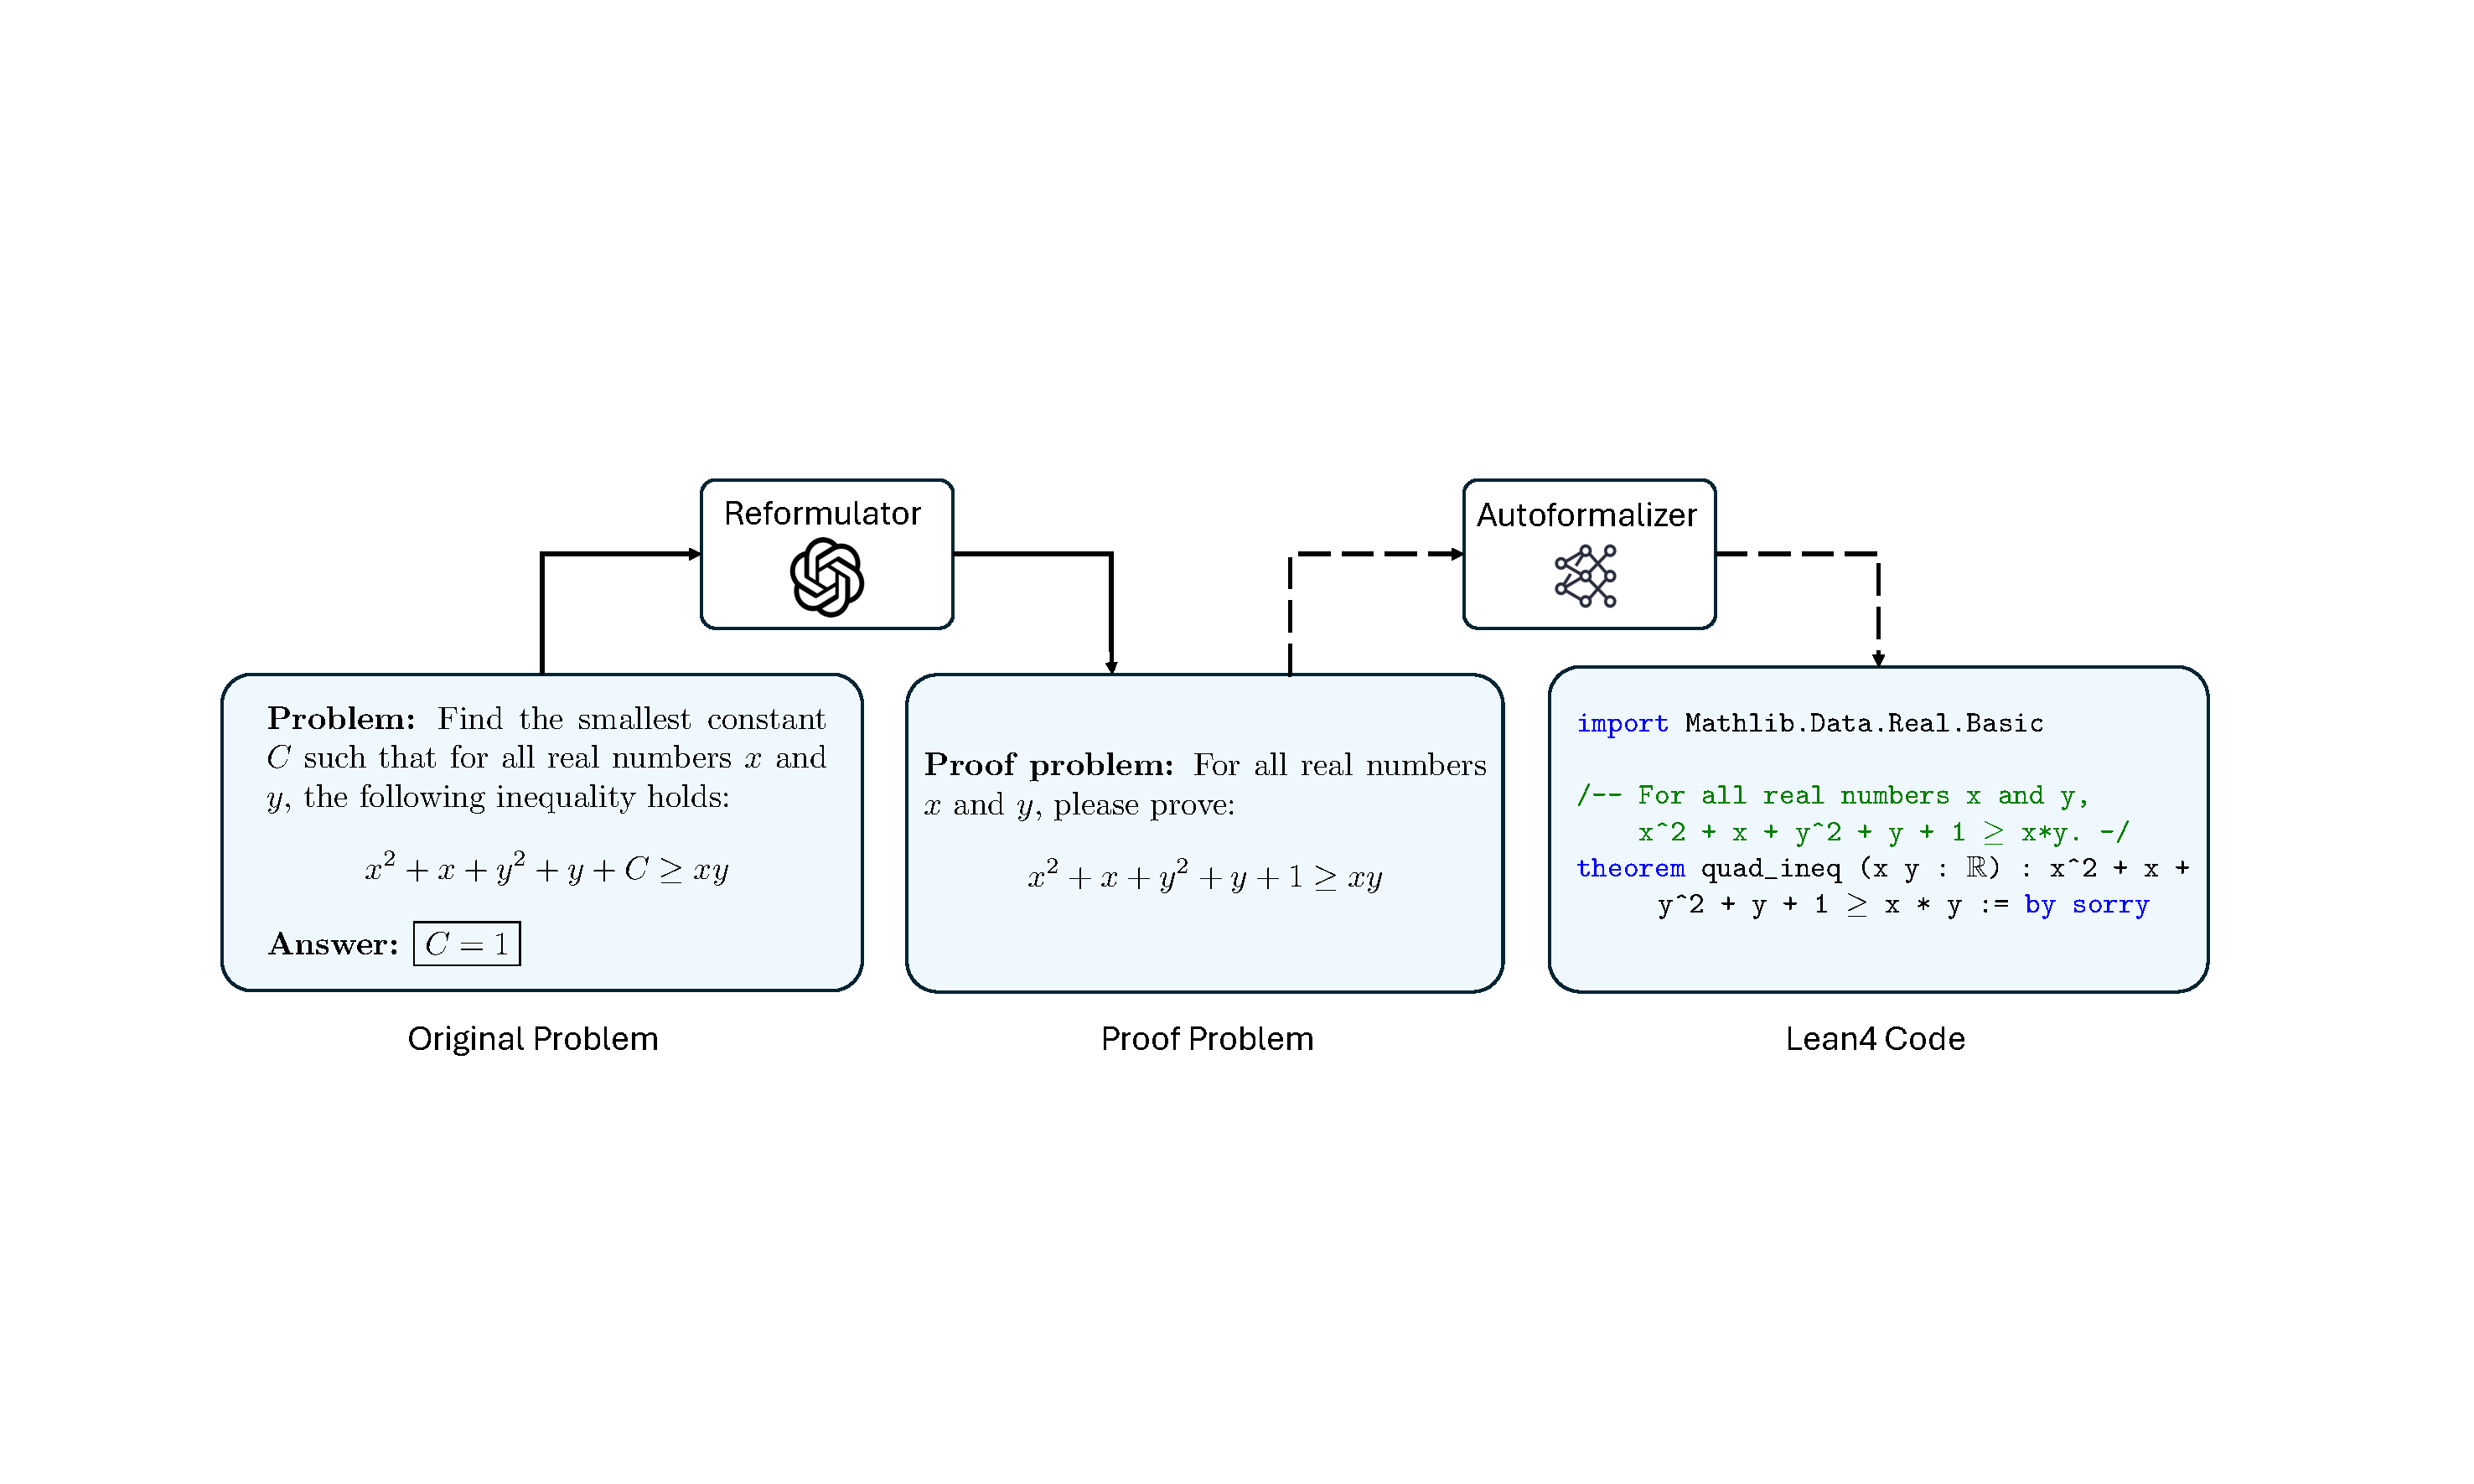
\includegraphics[width=1.0\linewidth]{figs/figure_formal_illustration_bound.pdf}
    \caption{Illustration of the formalization process for bound problems.}
    \label{fig:formal_illustration_bound}
\end{figure}

\begin{figure}[H]
    \centering
    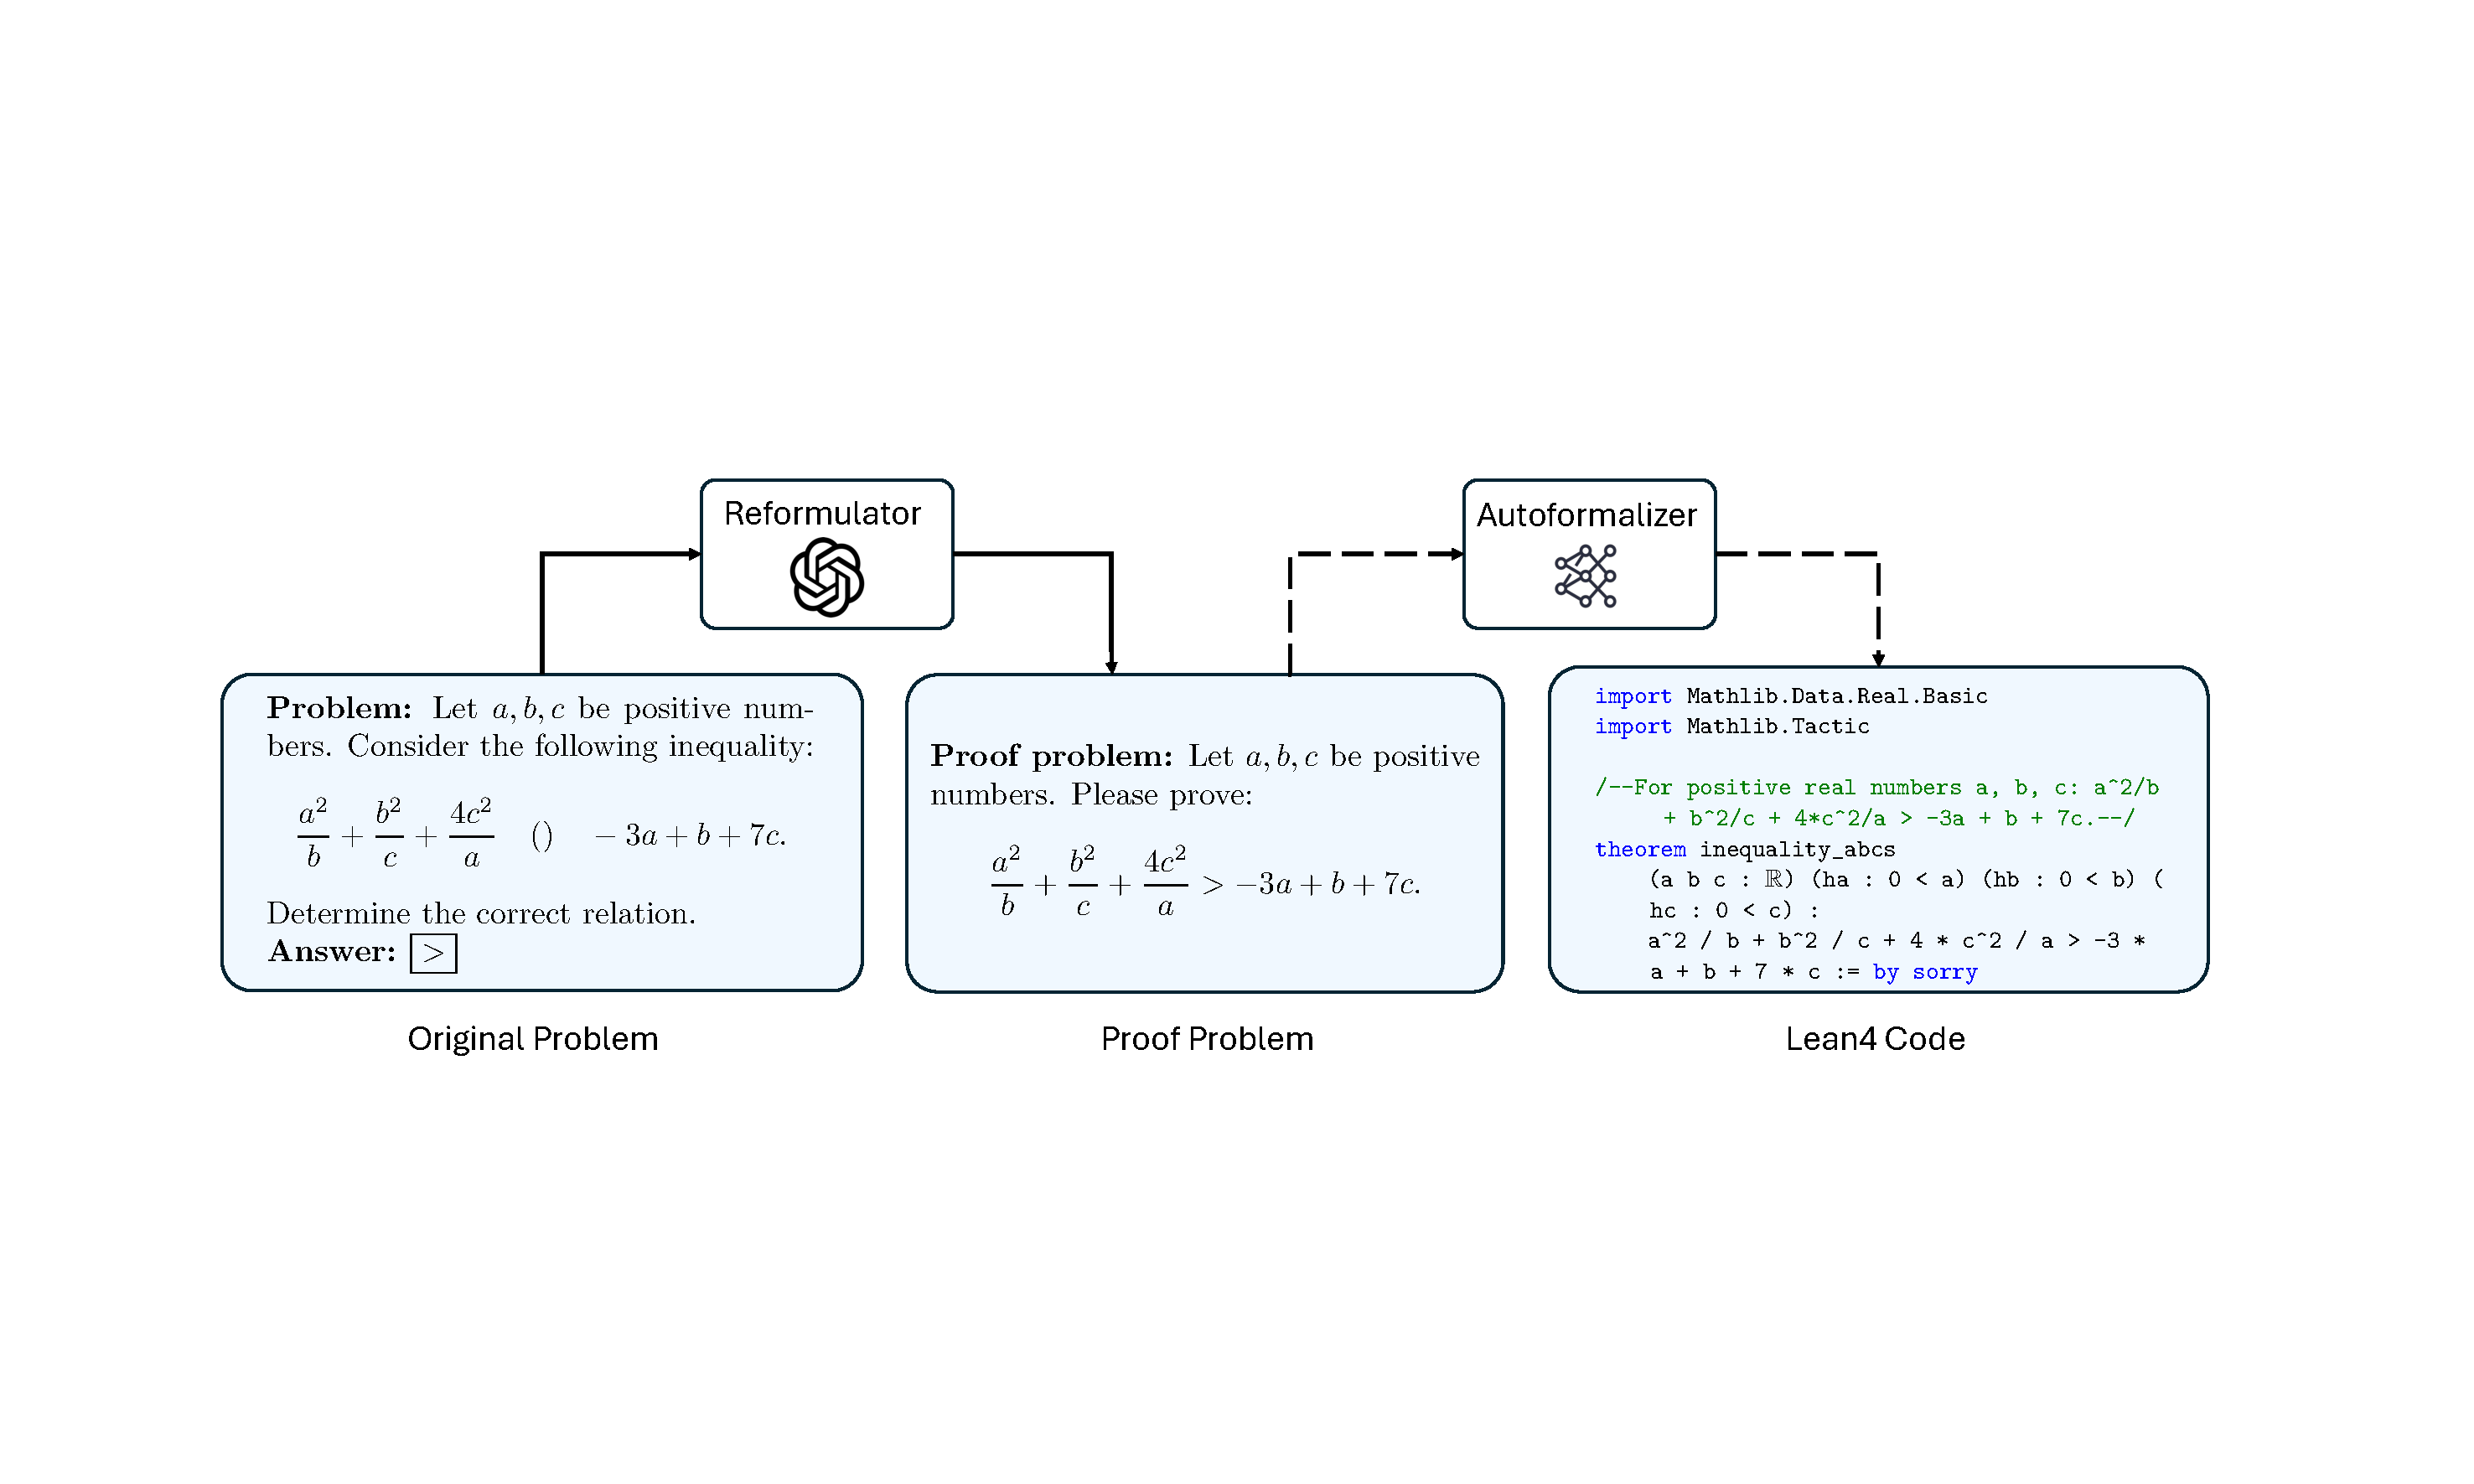
\includegraphics[width=1.0\linewidth]{figs/figure_formal_illustration_relation.pdf}
    \caption{Illustration of the formalization process for relation problems.}
    \label{fig:formal_illustration_relation}
\end{figure}

Once formalized, we evaluate SOTA ATP models on the Lean4 problems to measure their ability to solve inequality tasks. The results are as follows.

\begin{table}[H]
\centering
\small
\begin{tabular}{lc}
\toprule
\textbf{Model name} & \textbf{Pass rate (Pass@32)} \\
\midrule
DeepSeek-Prover-V2-7B~\cite{ren2025deepseek} & 6.0\%  \\
Kimina-Prover-Distill-8B~\cite{AI-MO_KiminaProverDistill8B} & 12.0\% \\
Goedel-Prover-V2-32B~\cite{lin2025goedelv2} & 13.0\% \\
Goedel-Prover-SFT~\cite{lin2025goedel}  & 14.0\% \\
\bottomrule
\end{tabular}
\vspace{2mm}
\caption{Pass@32 performance of state-of-the-art formal automated theorem proving models.}
\label{tab:table_formal_evaluation}
\vspace{-7mm}
\end{table}



The results in Table~\ref{tab:table_formal_evaluation} show that state-of-the-art (SOTA) formal automated theorem proving models still suffer from the difficult inequality problems in \dataset. Even the best-performing model, Goedel-Prover-SFT, achieves only a 14.0\% pass rate, while others remain far lower. This demonstrates that current approaches are inadequate for reliably solving the inequality-focused tasks presented in \dataset, and further methods are needed to achieve significant improvements in handling these challenging problems. 

% \clearpage
\subsubsection{Memorization Probe}
\label{app:memorization_probe}

To further demonstrate the modest degree of contamination in \dataset, we conducted a memorization probe experiment. In this probe, we systematically rephrased all test problems by swapping the terms on either side of each inequality and then re-evaluated models on the reformulated version. The rephrased problem is mathematically equivalent to the original one, differing only in presentation. This allows us to test whether models had merely memorized the original problems or could generalize to equivalent but rephrased tasks. Examples of the rephrased problems are as follows.

\begin{examplebox}[Memorization Probe Reformulation Example 1: Bound Problem]

\textbf{Original Problem:} Find the smallest constant $C$ such that for all real numbers $x$ and $y$, the following inequality holds:
$$
x^2 + x + y^2 + y + C \geq x y
$$

\textbf{Original Answer:} $\boxed{C=1}$ \\

\textbf{Rephrased Problem:} Find the smallest constant $C$ such that for all real numbers $x$ and $y$, the following inequality holds:
$$
 x y \leq x^2 + x + y^2 + y + C 
$$

\textbf{Rephrased Answer:} $\boxed{C=1}$

\end{examplebox}
\begin{examplebox}[Memorization Probe Reformulation Example 2: Relation Problem]

\textbf{Original Problem:} Let $a, b, c$ be positive numbers. Consider the following inequality:
$$
\frac{a^2}{b} + \frac{b^2}{c} + \frac{4c^2}{a} \quad () \quad -3a + b + 7c.
$$

Determine the correct inequality relation to fill in the blank.

Options: (A) $\leq$ \quad(B) $\geq$ \quad (C) $=$  \quad (D) $<$ \quad  (E) $>$  \quad (F) None of the above\\

\textbf{Original Answer:} $\boxed{\text{(E)} >}$ \\

\textbf{Rephrased Problem:}  Let $a, b, c$ be positive numbers. Consider the following inequality:
$$
 -3a + b + 7c  \quad () \quad\frac{a^2}{b} + \frac{b^2}{c} + \frac{4c^2}{a}.
$$

Determine the correct inequality relation to fill in the blank.

Options: (A) $\leq$ \quad(B) $\geq$ \quad (C) $=$  \quad (D) $<$ \quad  (E) $>$  \quad (F) None of the above\\

\textbf{Rephrased Answer:}  $\boxed{\text{(D)} <}$

\end{examplebox}

We evaluate Claude Sonnet 4, GPT-4.1 mini, and o4-mini on both the original and reformulated versions of the \dataset test set, with their performance results summarized below.

As shown in Figures~\ref{fig:memorization_probe_overall_acc} and \ref{fig:memorization_probe_answer_acc}, model performance remains largely consistent across the original and reformulated versions of the \dataset test set. For example, GPT-4.1 mini maintains an overall accuracy of 8.5\% in both conditions, while o4-mini shows only a slight drop from 15.5\% to 15.0\%. In terms of answer accuracy, Claude Sonnet 4 decreases modestly from 44.0\% to 40.0\%, whereas o4-mini remains steady at 65.0\%. These small shifts—generally under 5 percentage points—indicate that the models adapt well to rephrased tasks rather than relying on memorized solutions. This provides strong evidence that contamination is unlikely, as performance is not driven by rote recall.

\clearpage

\begin{figure}[H]
    \centering
    \begin{minipage}{0.485\textwidth}
        \centering
        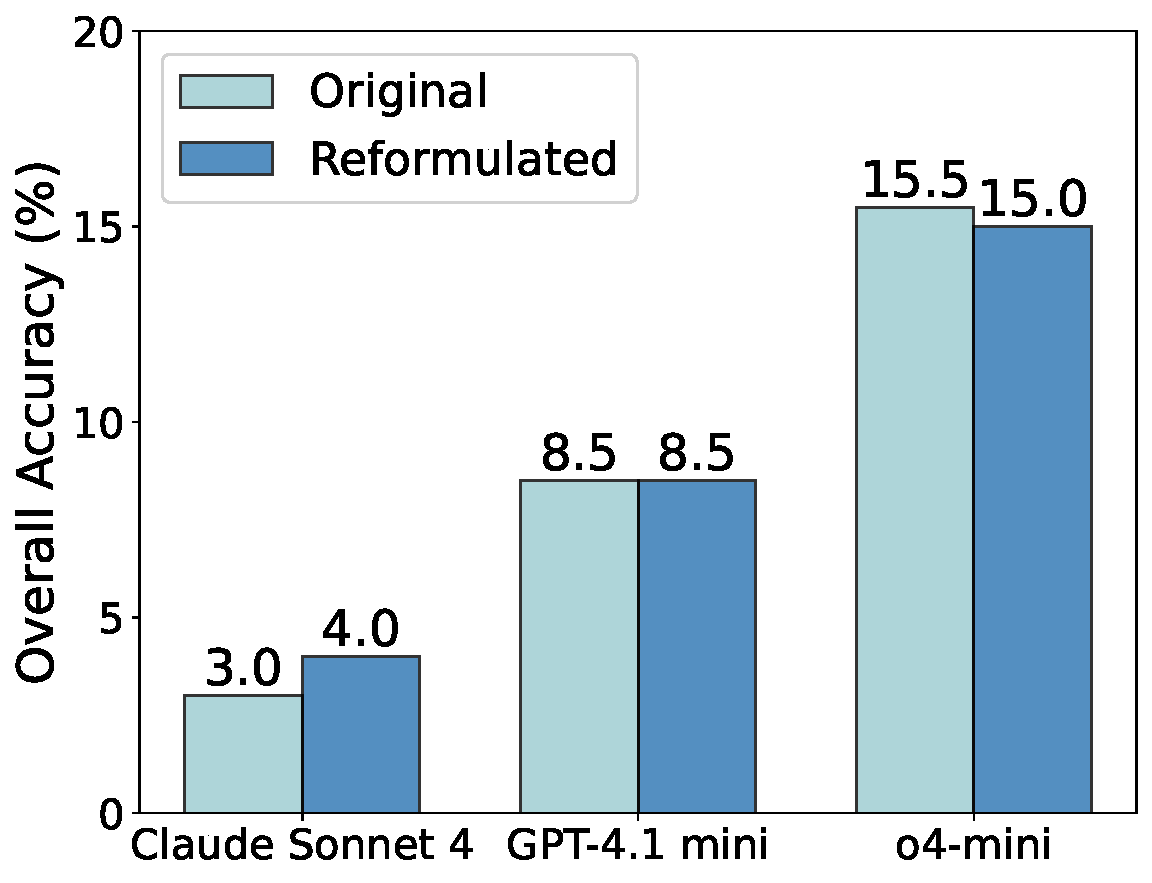
\includegraphics[width=0.9\linewidth]{figs/memorization_probe_overall_acc_figure.pdf}
        \caption{Model performance on the original and reformulated version of the \dataset test set (\textit{Overall Accuracy}).}
        \label{fig:memorization_probe_overall_acc}
    \end{minipage}
    \hfill
    \begin{minipage}{0.485\textwidth}
        \centering
        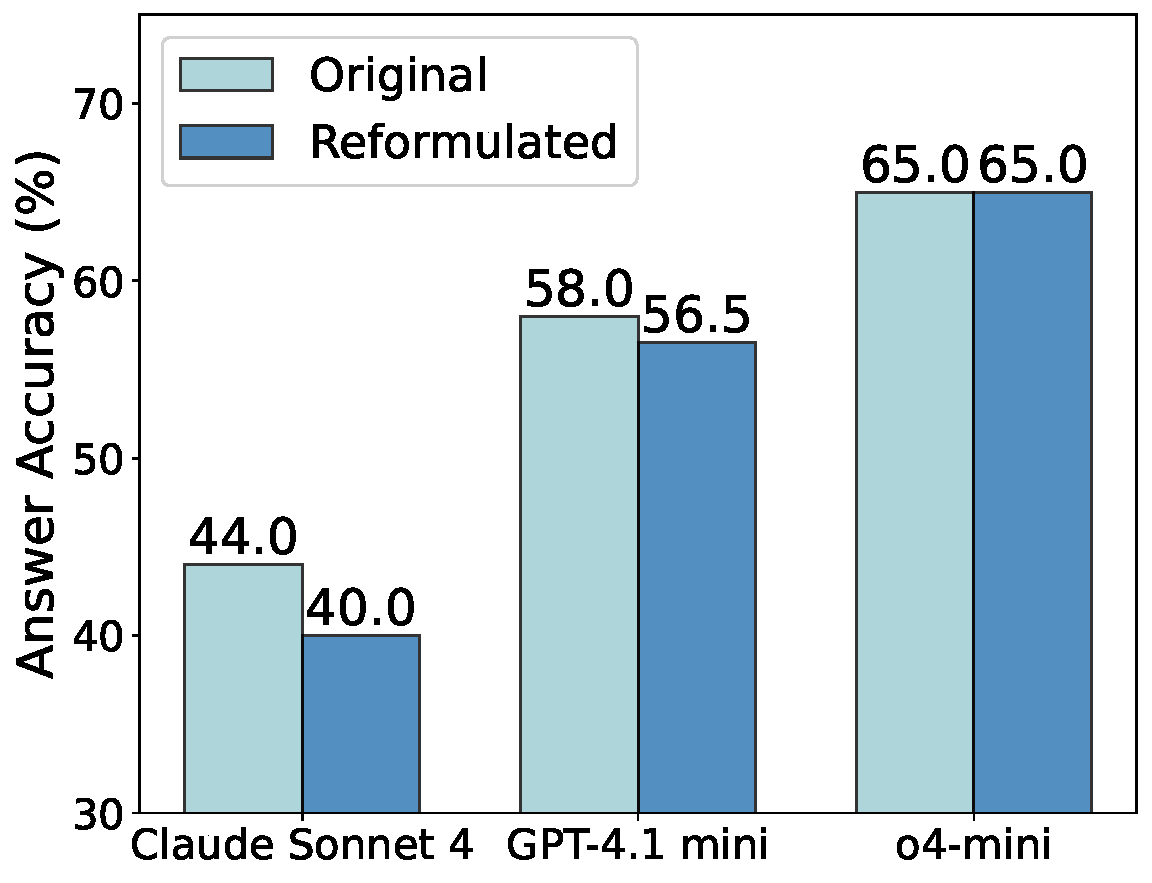
\includegraphics[width=0.9\linewidth]{figs/memorization_probe_answer_acc_figure.pdf}
        \caption{Model performance on the original and reformulated version of the \dataset test set (\textit{Answer Accuracy}).}
        \label{fig:memorization_probe_answer_acc}
    \end{minipage}
    \vspace{-3mm}
\end{figure}





% \clearpage
\subsection{Limitations} 
\label{app:limitations}

While our work introduces a novel dataset and evaluation judges for LLM-based inequality proving, we acknowledge several limitations that warrant discussion and offer avenues for future research.

\subparagraph{Potential for data contamination.} Although we took significant measures to mitigate data leakage by commissioning novel test problems curated by experts, keeping ground truth answers private, and utilizing an online leaderboard for evaluation, a residual risk of contamination remains. LLMs possess vast training corpora, and it is possible they have encountered problems with similar structures or underlying principles during pre-training, potentially inflating performance beyond true generalization capabilities. Our expert curation and review process aimed to minimize this, but perfect isolation from prior knowledge is challenging to guarantee.

\subparagraph{Training dataset scale and scope.} The \dataset training set, while meticulously curated with 1,252 problems featuring step-wise solutions, multiple solution paths, and theorem annotations, is modest in size compared to the massive datasets often used for pre-training or fine-tuning large models. We prioritized quality and depth (step-wise solutions, theorems) to the challenging Olympiad-level domain over sheer quantity. While sufficient for benchmarking current models, post-training, and exploring test-time techniques, this scale might be insufficient for training highly specialized models from scratch or for capturing the full diversity of inequality types. Future work could focus on scaling up the dataset while maintaining quality, potentially through community contributions.

\subparagraph{Inherent inaccuracies in LLM-as-judge evaluation.} Our \textit{LLM-as-judge} framework demonstrates high reliability on our development set (F1$=1.0$ for the \textit{final-answer judge}, $>0.9$ average for step-wise judges). However, while significantly more scalable than human expert evaluation, these judges are still imperfect. As illustrated by examples in \S\ref{app:judge_failure_examples}, they can occasionally misinterpret complex reasoning, overlook subtle logical flaws, or fail to correctly assess nuanced mathematical arguments. The current set of step-wise judges targets common failure modes but does not cover all possible error types, such as the correctness of complex symbolic transformations or the optimal choice of strategy. Potential improvements include using more powerful (but potentially more expensive) LLMs as judge backends (e.g., o3), developing specialized judges trained on annotated errors, or adding judges for specific mathematical operations like symbolic manipulation verification.

\subparagraph{Mitigation, not elimination, of answer guessability.} 
The inclusion of step-wise judges significantly mitigates the issue of models guessing the correct final answer without sound reasoning. However, it does not eliminate this possibility entirely. A model might still arrive at the correct bound or relation through chance or heuristics and support it with plausible-sounding, yet flawed, intermediate steps capable of misleading one or more judges. The requirement to pass all judges reduces this risk, but the fundamental challenge of distinguishing genuine mathematical insight from convincing yet spurious reasoning remains.

\subparagraph{Computational cost of evaluation.} While more efficient than manual expert grading, our multi-judge evaluation protocol is computationally more intensive than simple final-answer checking (e.g., string matching). Evaluating each solution requires multiple LLM inferences (one for the final answer, four for step-wise checks). This cost scales linearly with the number of models and problems being evaluated and could become a factor in very large-scale benchmarking efforts.


\subsection{Broader Impacts}
\label{app:impacts}

This research focuses on advancing the mathematical reasoning capabilities of LLMs, specifically in the domain of inequality proving. While the work is primarily foundational and unlikely to lead directly to malicious applications such as disinformation or surveillance, potential negative societal impacts could arise from the misuse or misinterpretation of the technology. The most significant risk stems from over-reliance on LLM-generated proofs that may appear correct superficially (achieving high answer accuracy) but contain critical logical flaws, as demonstrated by the sharp drop in performance under our step-wise evaluation. If such flawed proofs were uncritically accepted in fields requiring mathematical rigor, such as scientific modeling, engineering design, or financial analysis, they could lead to incorrect conclusions, faulty systems, or economic miscalculations. Our contribution of a rigorous, step-wise evaluation methodology serves as a potential mitigation strategy by promoting transparency and enabling the identification of fragile reasoning chains, thereby encouraging cautious deployment and emphasizing the need for verification, especially in high-stakes applications. The public release of the \dataset benchmark further supports community efforts in understanding and improving the reliability of LLM reasoning.
